\chapter{Supplementary Graphs and Tables}
\section{Supplementary Graphs}
\subsection{Winning ration plots for simple network topologies}
\label{append:wining-ratio-further-plot}
In this section, as explained in \autoref{sub:winning-ratio}, winning ratio point plots
have been conducted. These point plots can be found below.
\begin{figure}[H]
	\centering
	\begin{subfigure}[t]{0.75\textwidth}
		\centering
		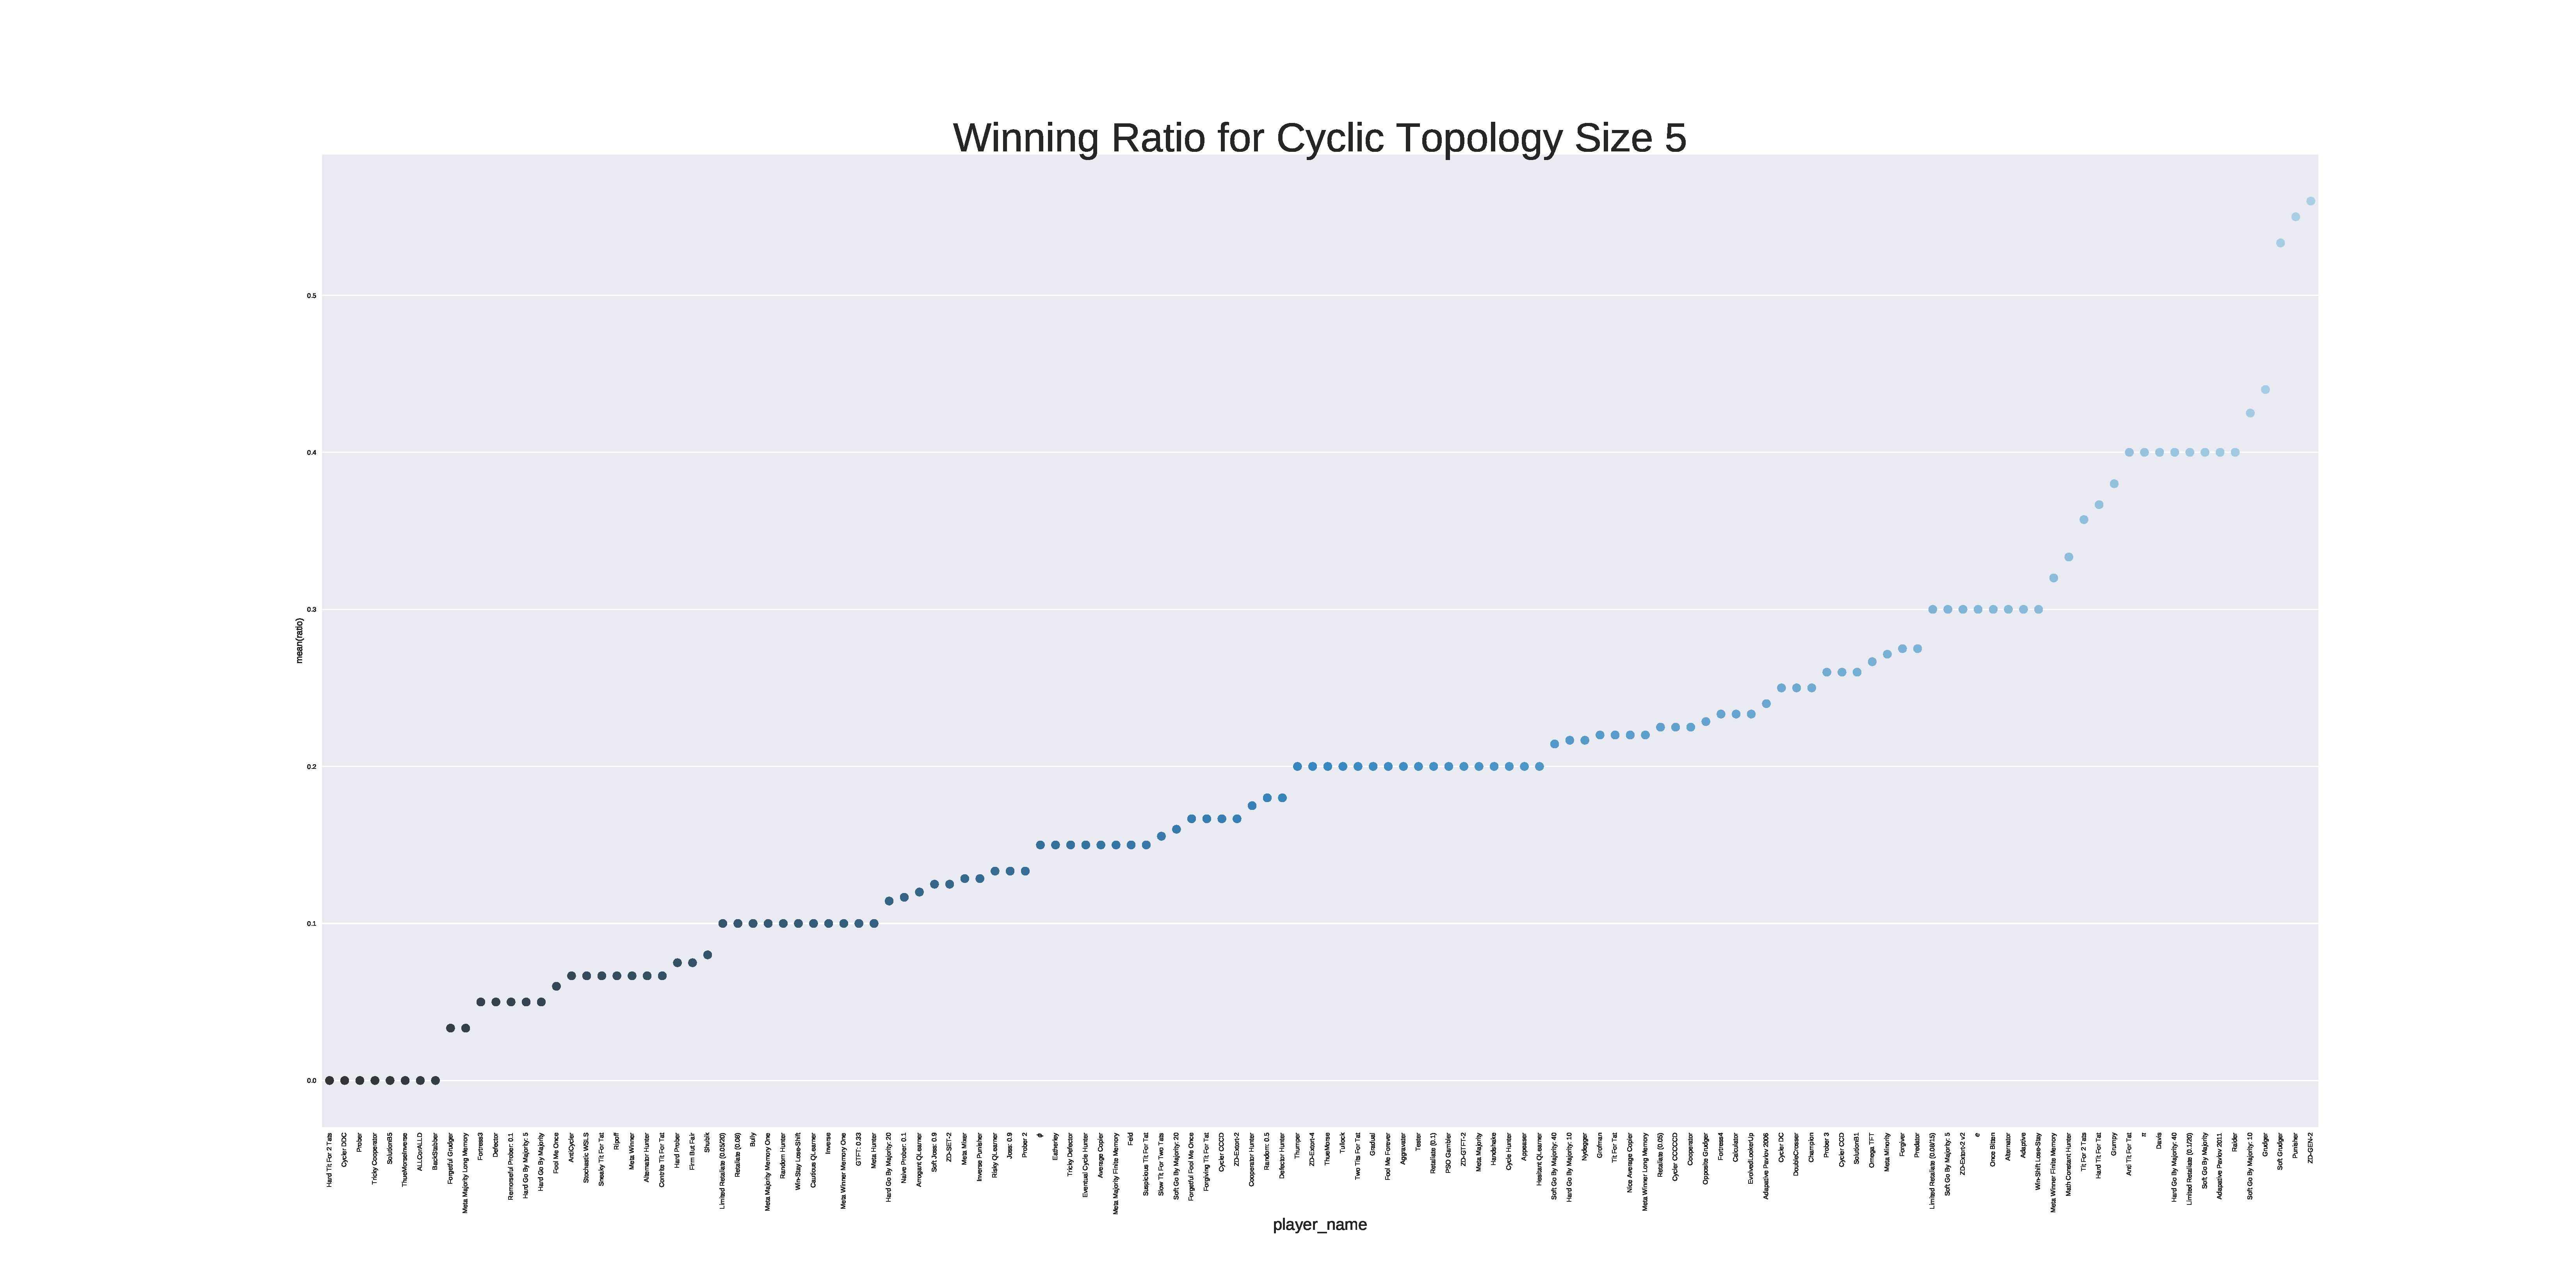
\includegraphics[width=\linewidth]{appendix/winners-Cyclic-5.pdf}
		\caption{Winning ratio cyclic topology size 5}
	\end{subfigure}
	\hfill
	\begin{subfigure}[t]{0.75\textwidth}\centering
		\centering
		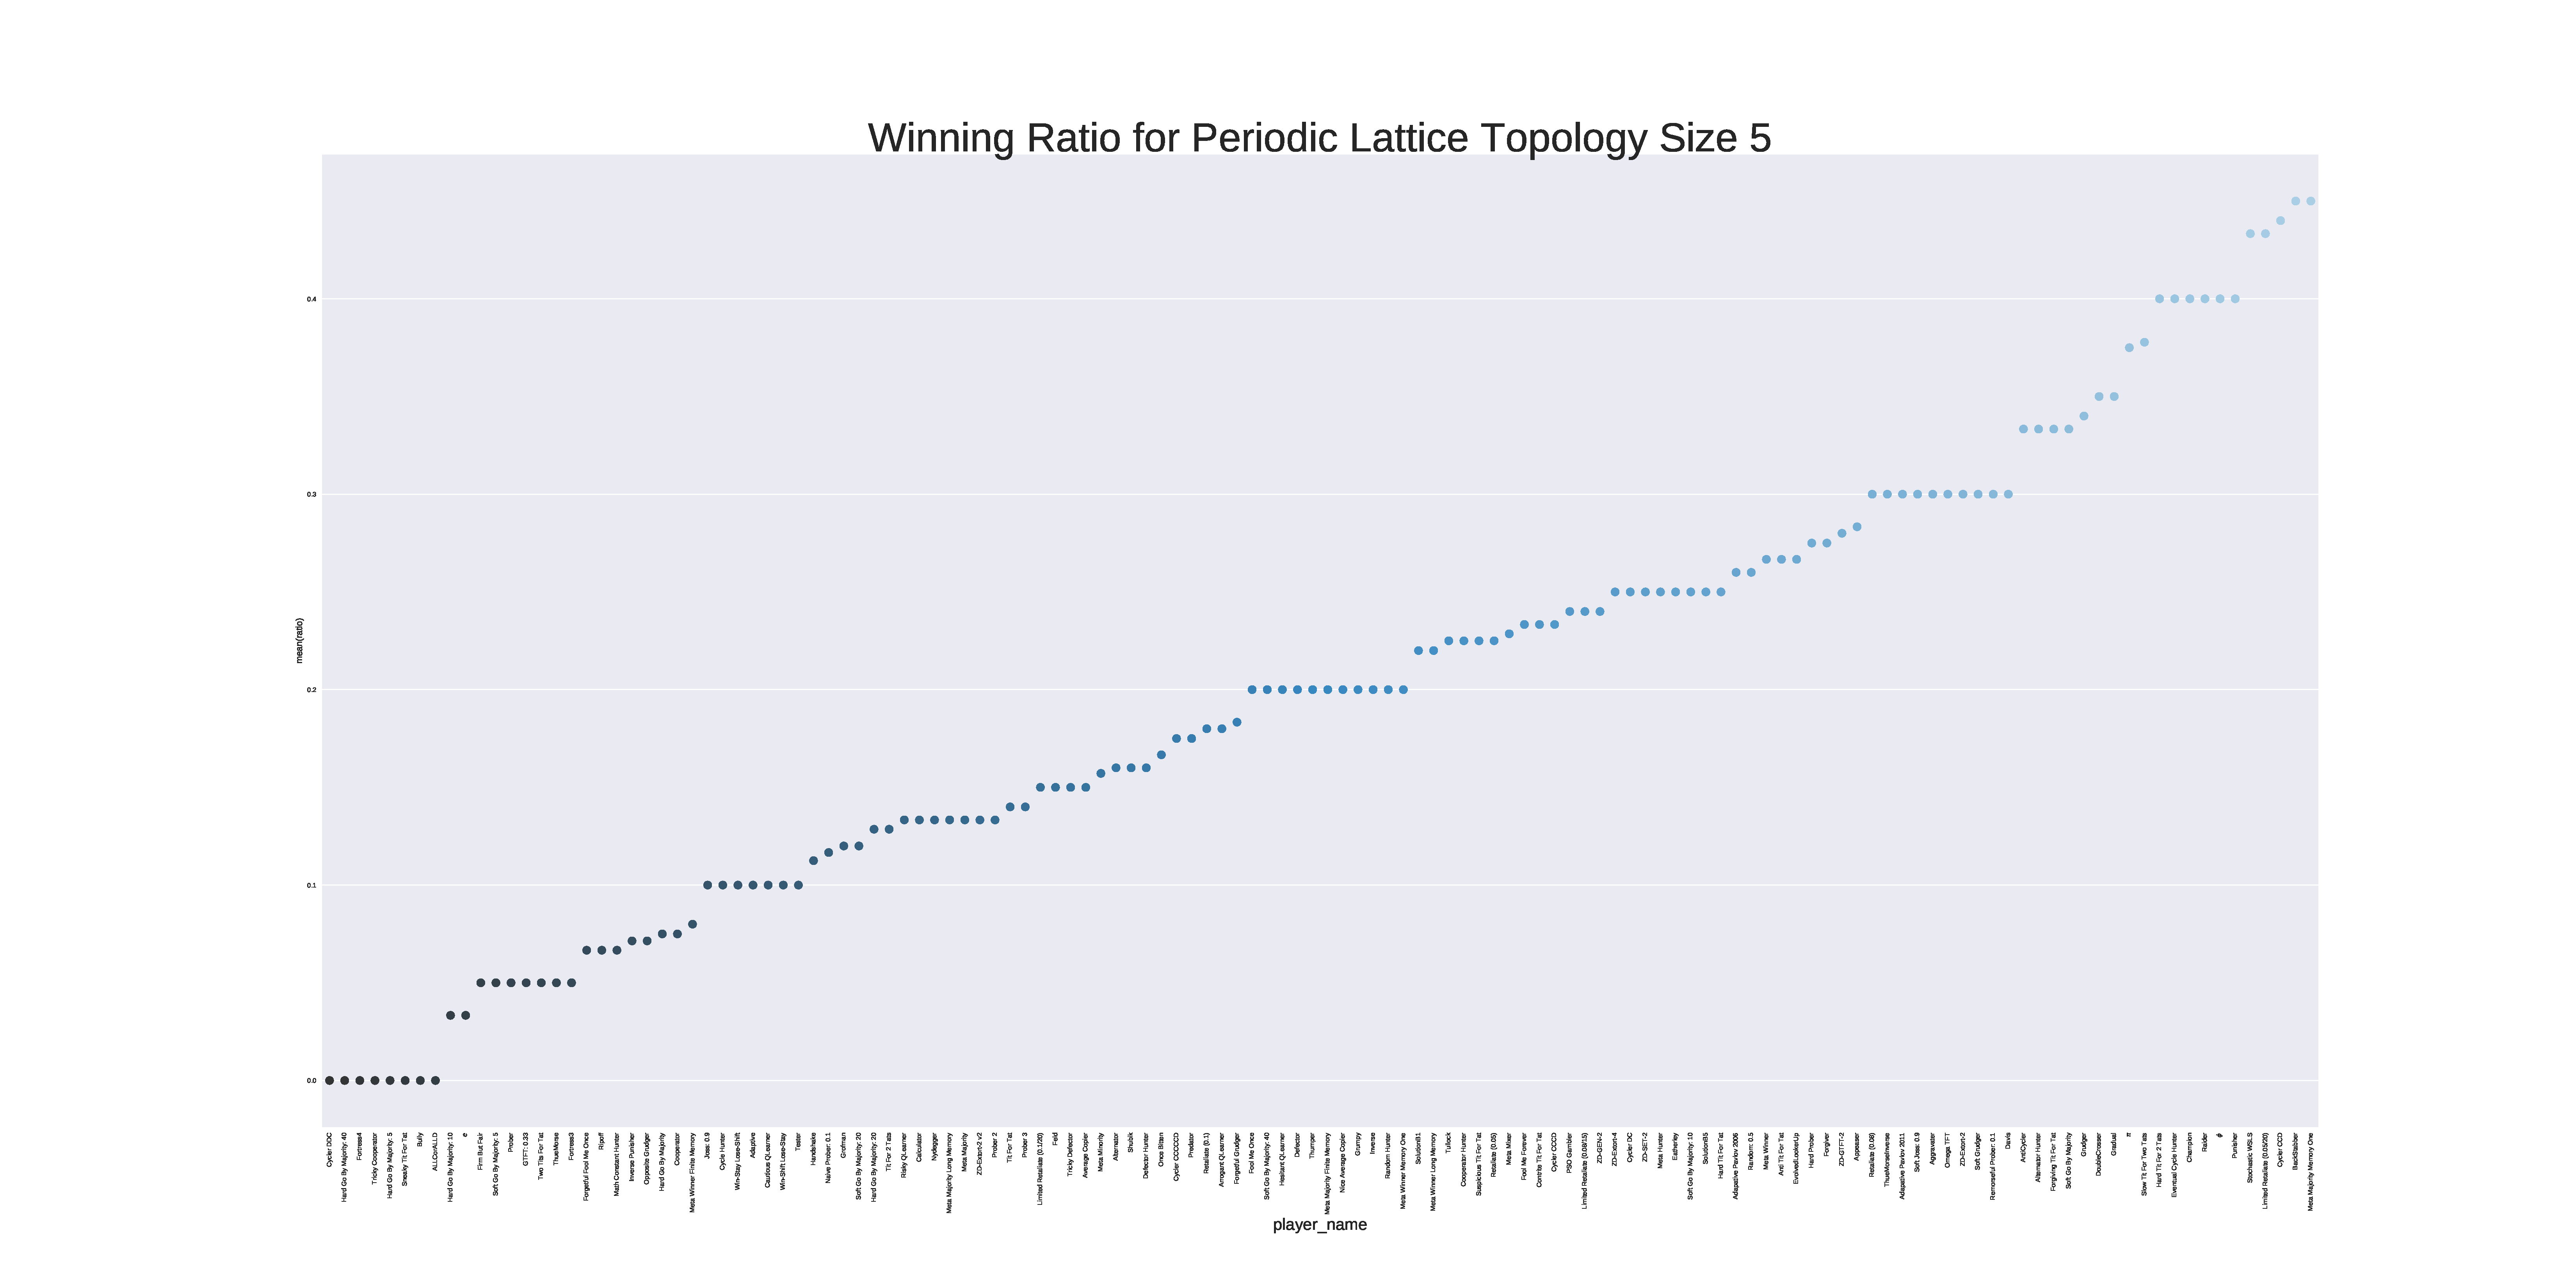
\includegraphics[width=\linewidth]{appendix/winners-Periodic-Lattice-5.pdf}
		\caption{Winning ratio periodic lattice topology size 5}
	\end{subfigure}
	\hfill
	\begin{subfigure}[t]{0.75\textwidth}\centering
		\centering
		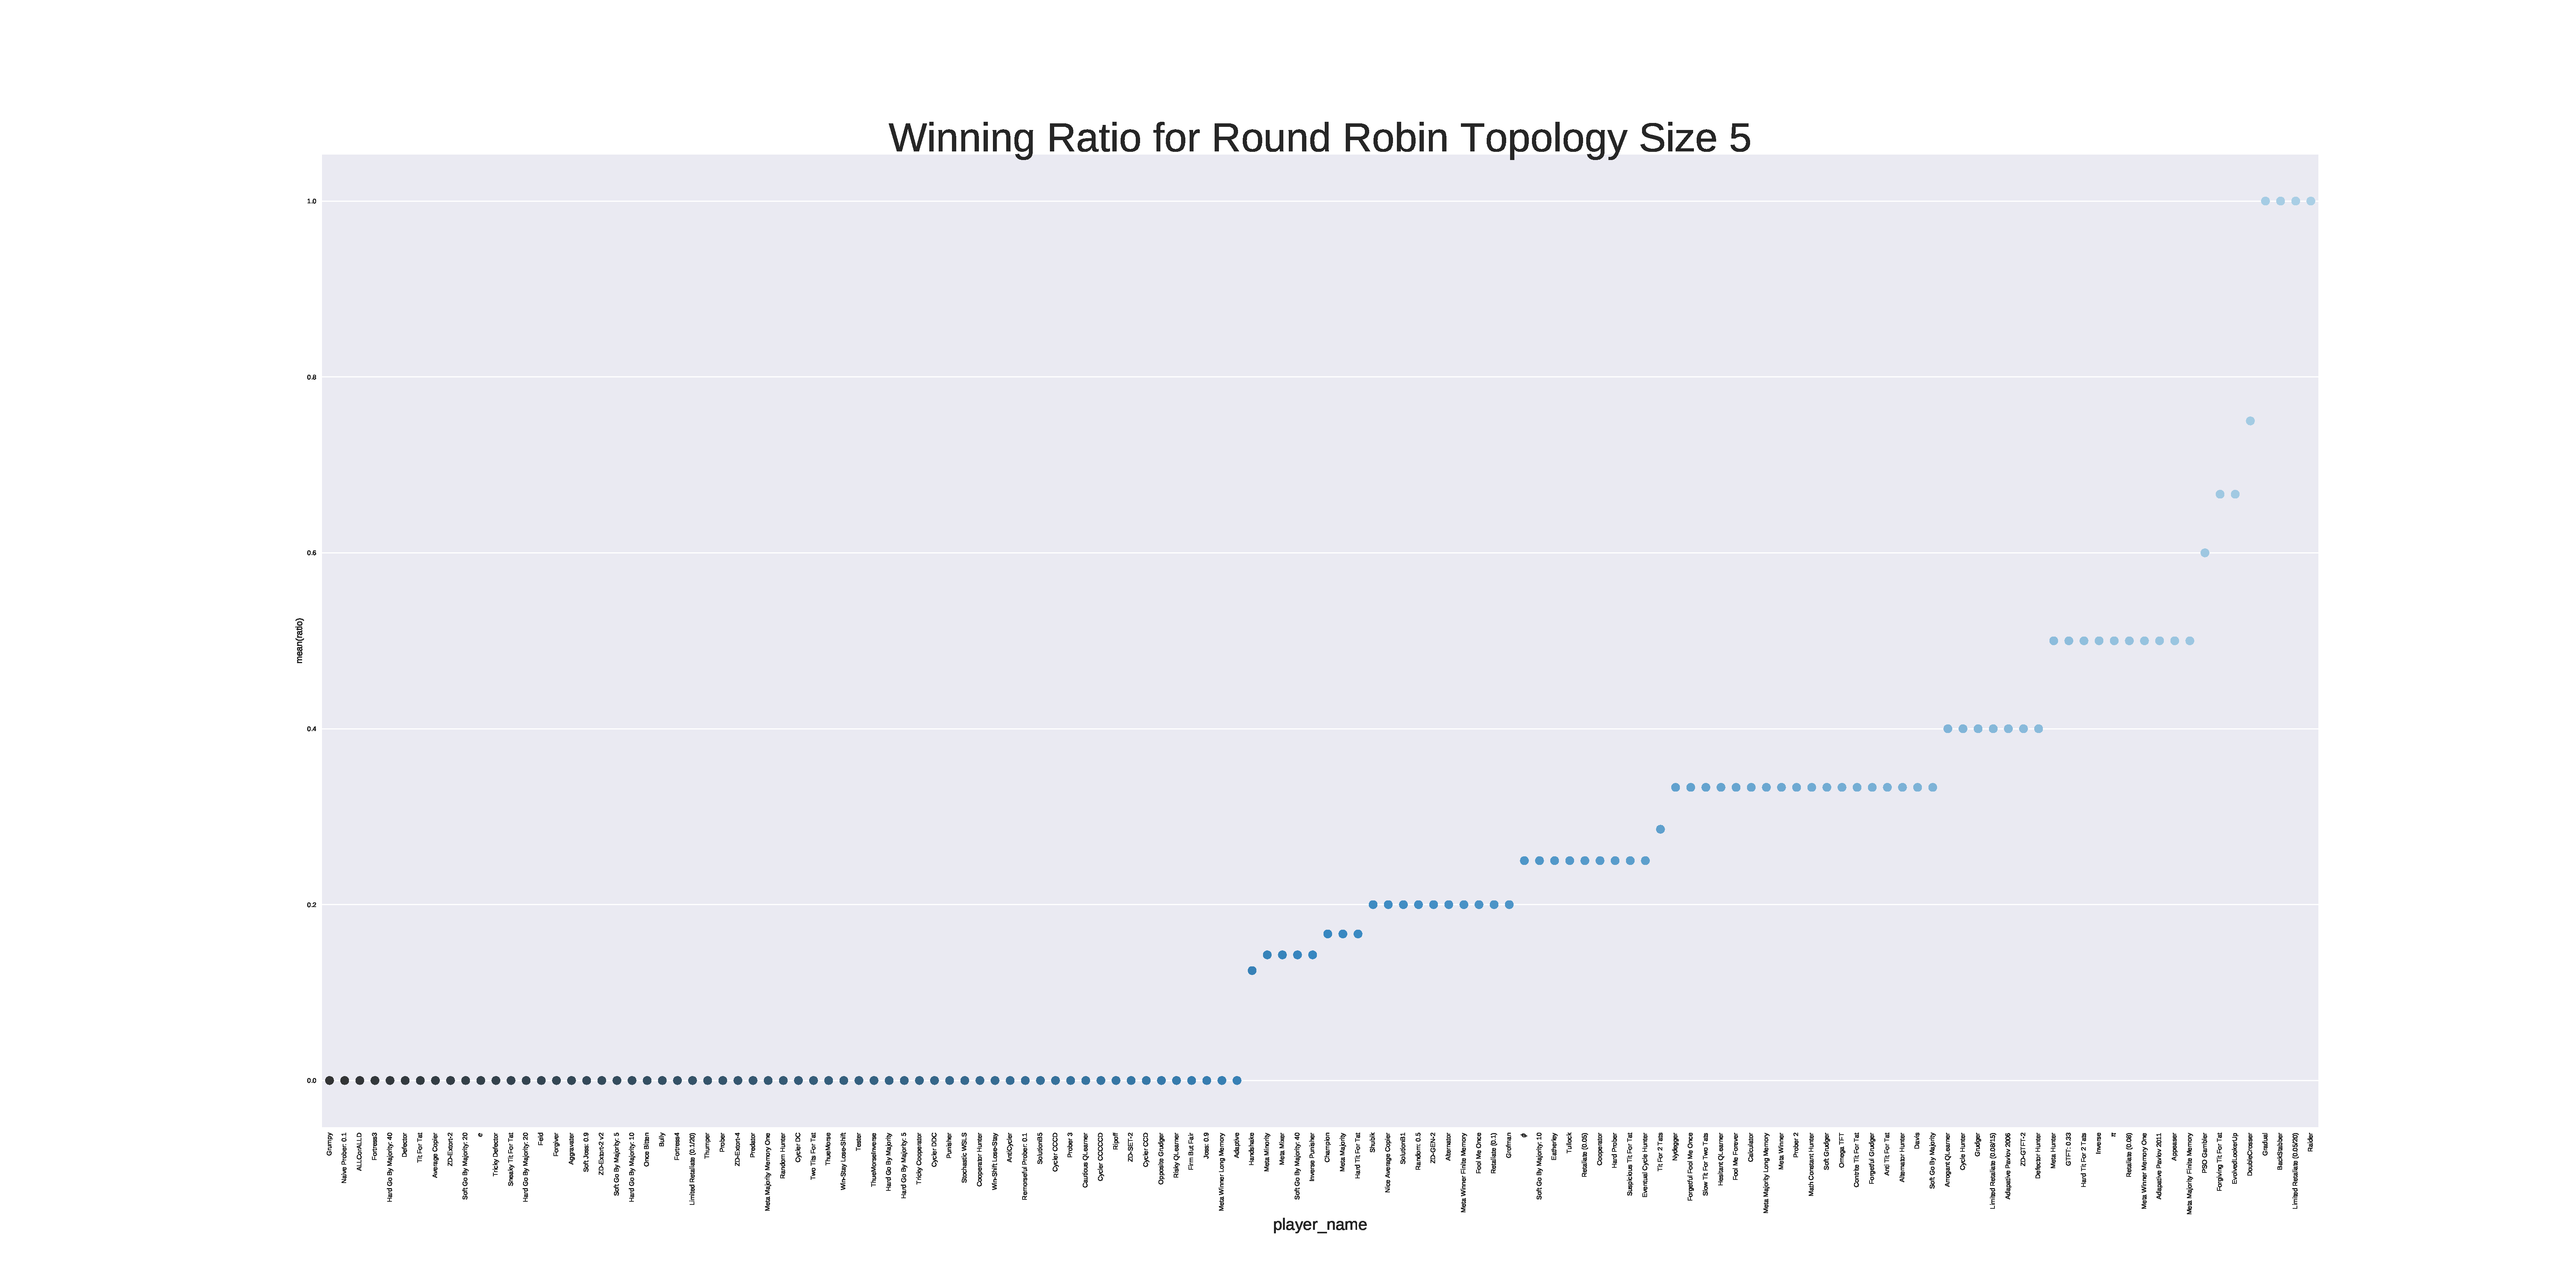
\includegraphics[width=\linewidth]{appendix/winners-Round-Robin-5.pdf}
		\caption{Winning ratio round robin topology size 5}
	\end{subfigure}
	\caption{Winning ratio for all three topologies size 5}
	\label{fig:winning-five}

\end{figure}

\begin{figure}[H]
	\centering
	\begin{subfigure}[t]{0.75\textwidth}
		\centering
		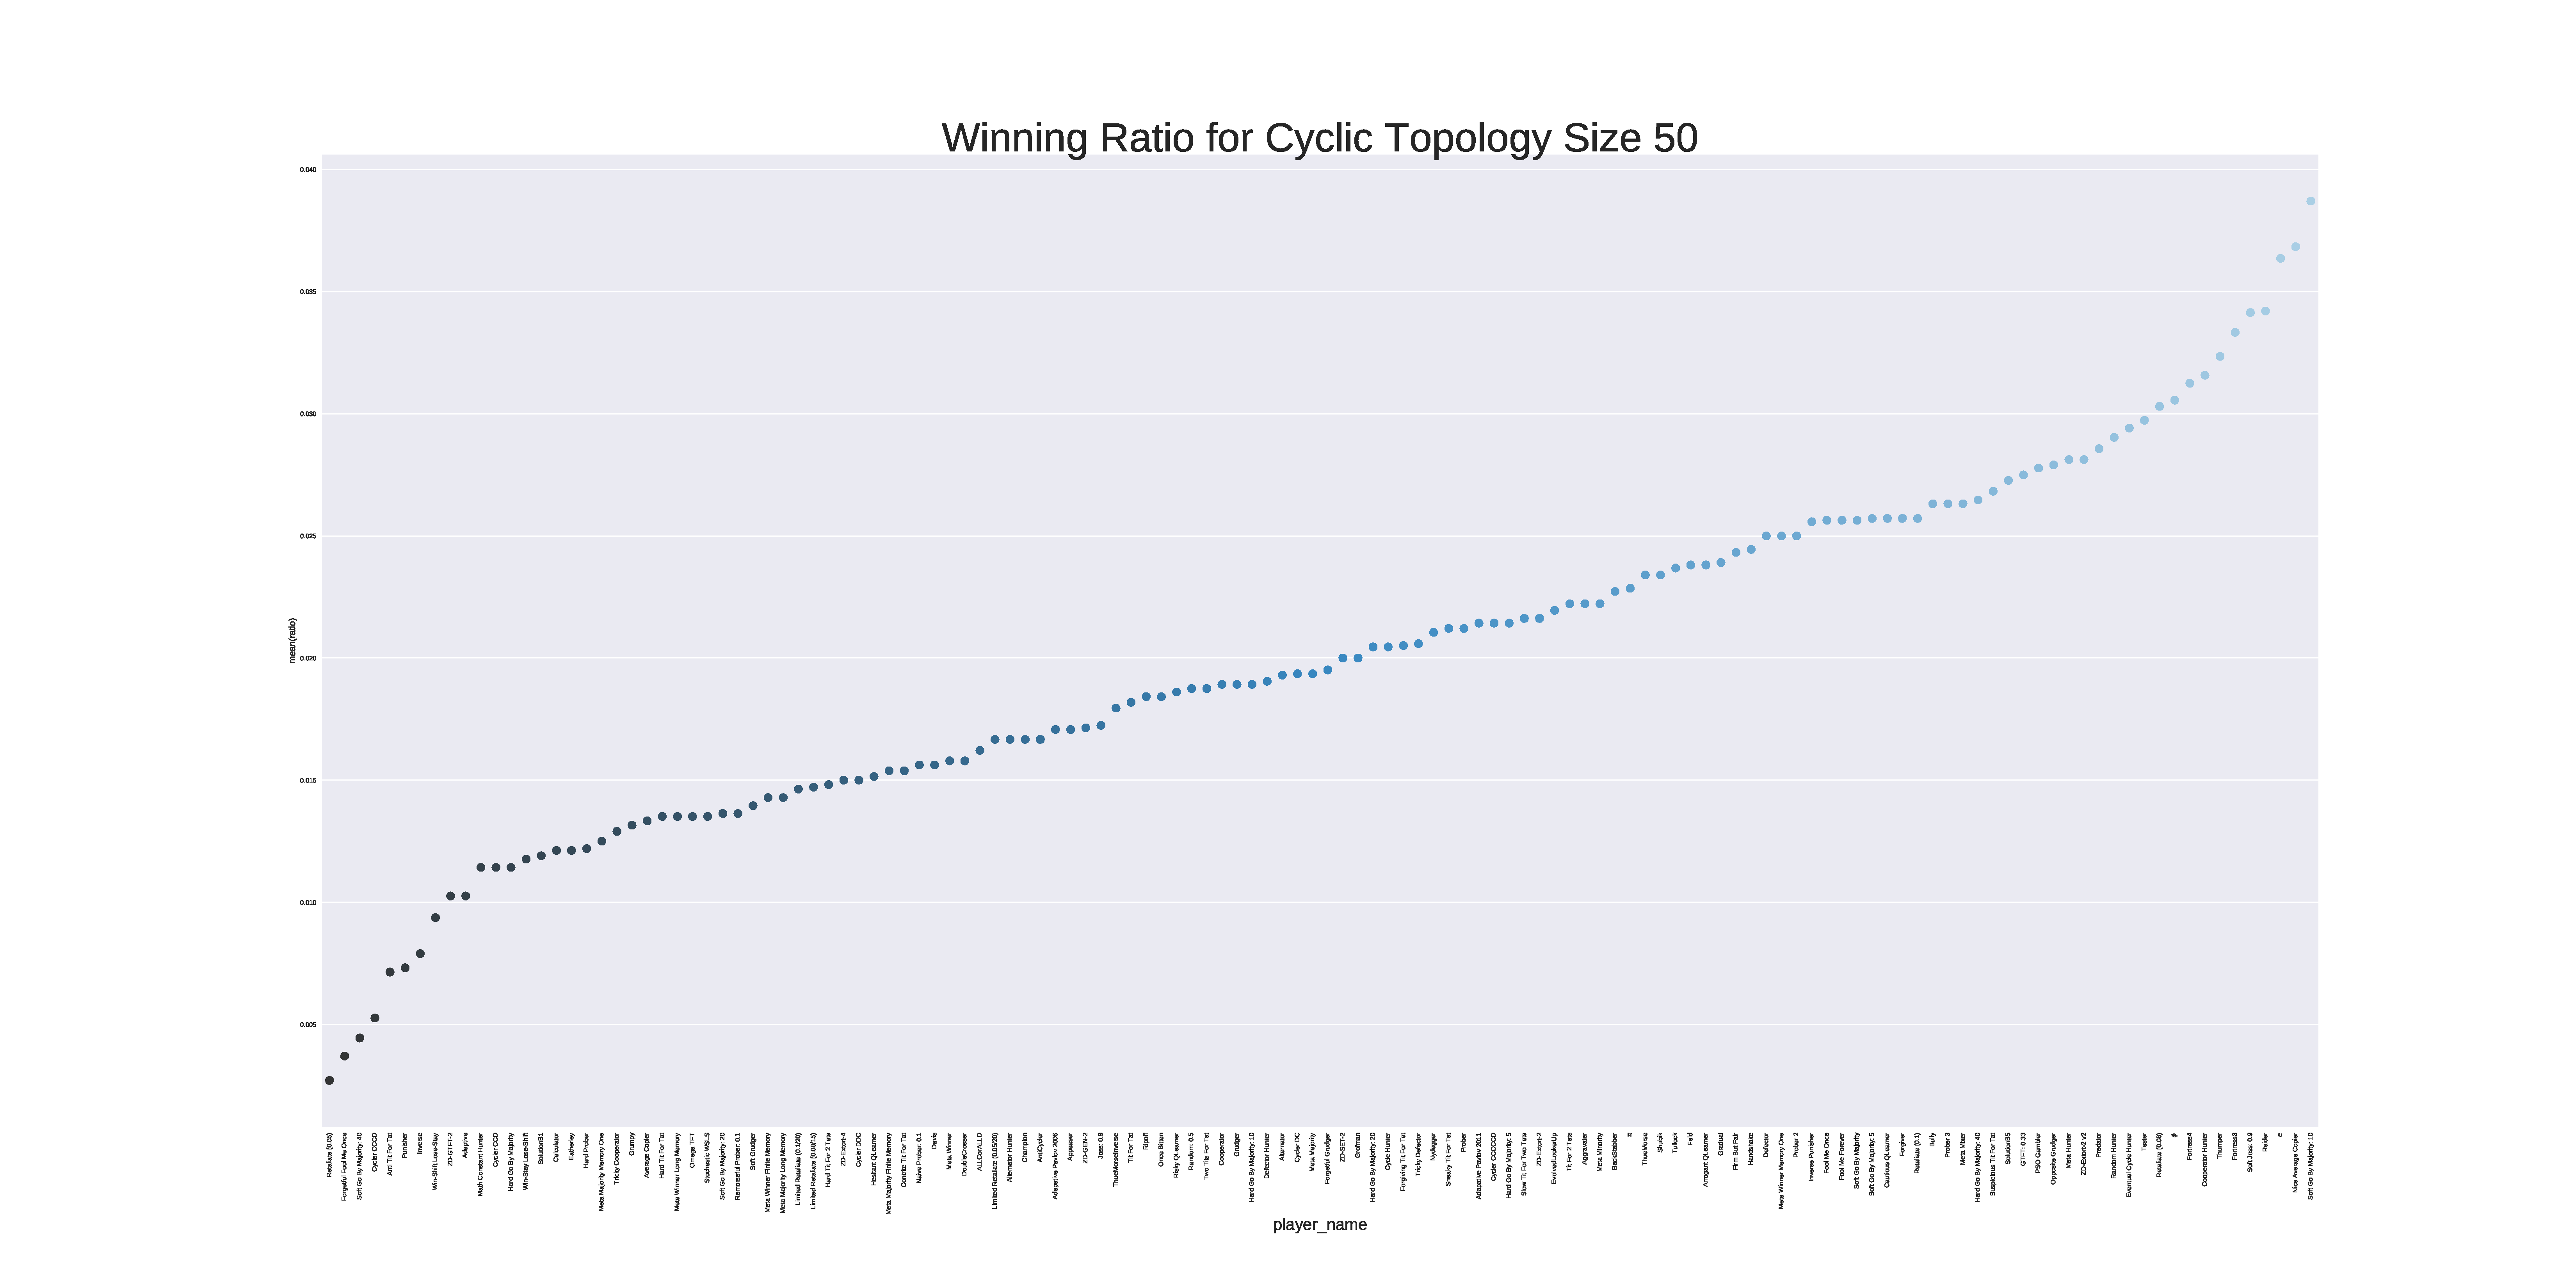
\includegraphics[width=\linewidth]{appendix/winners-Cyclic-50.pdf}
		\caption{Winning ratio cyclic topology size 50}
	\end{subfigure}
	\hfill
	\begin{subfigure}[t]{0.75\textwidth}\centering
		\centering
		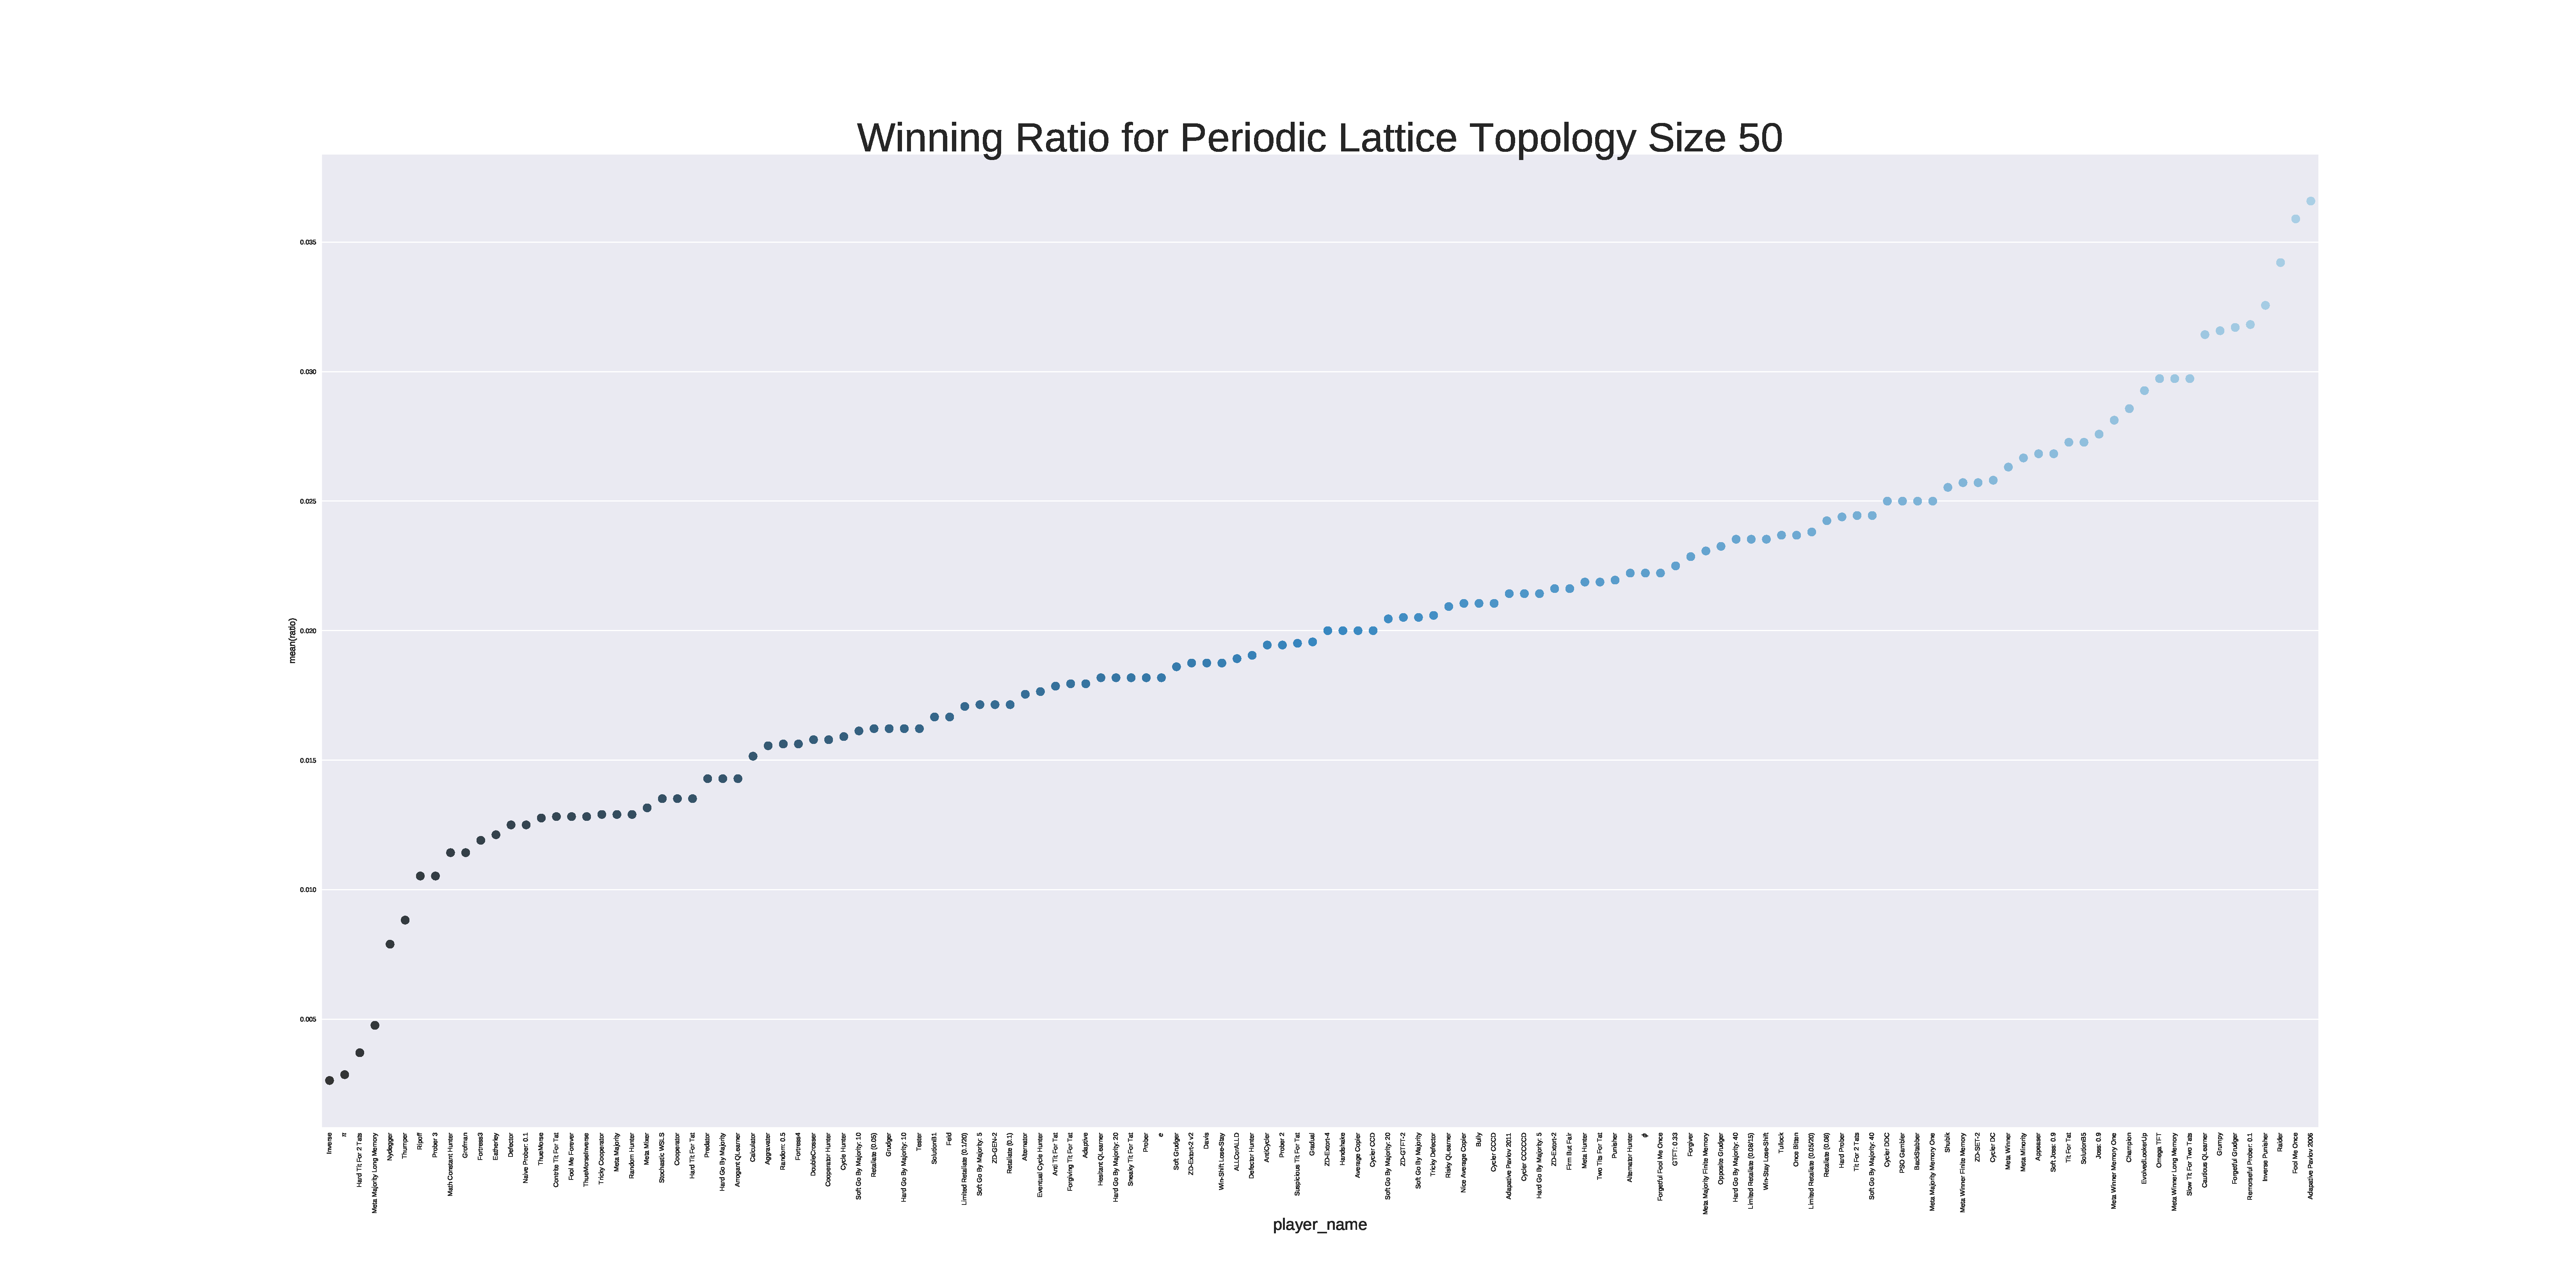
\includegraphics[width=\linewidth]{appendix/winners-Periodic-Lattice-50.pdf}
		\caption{Winning ratio periodic lattice topology size 50}
	\end{subfigure}
	\hfill
	\begin{subfigure}[t]{0.75\textwidth}\centering
		\centering
		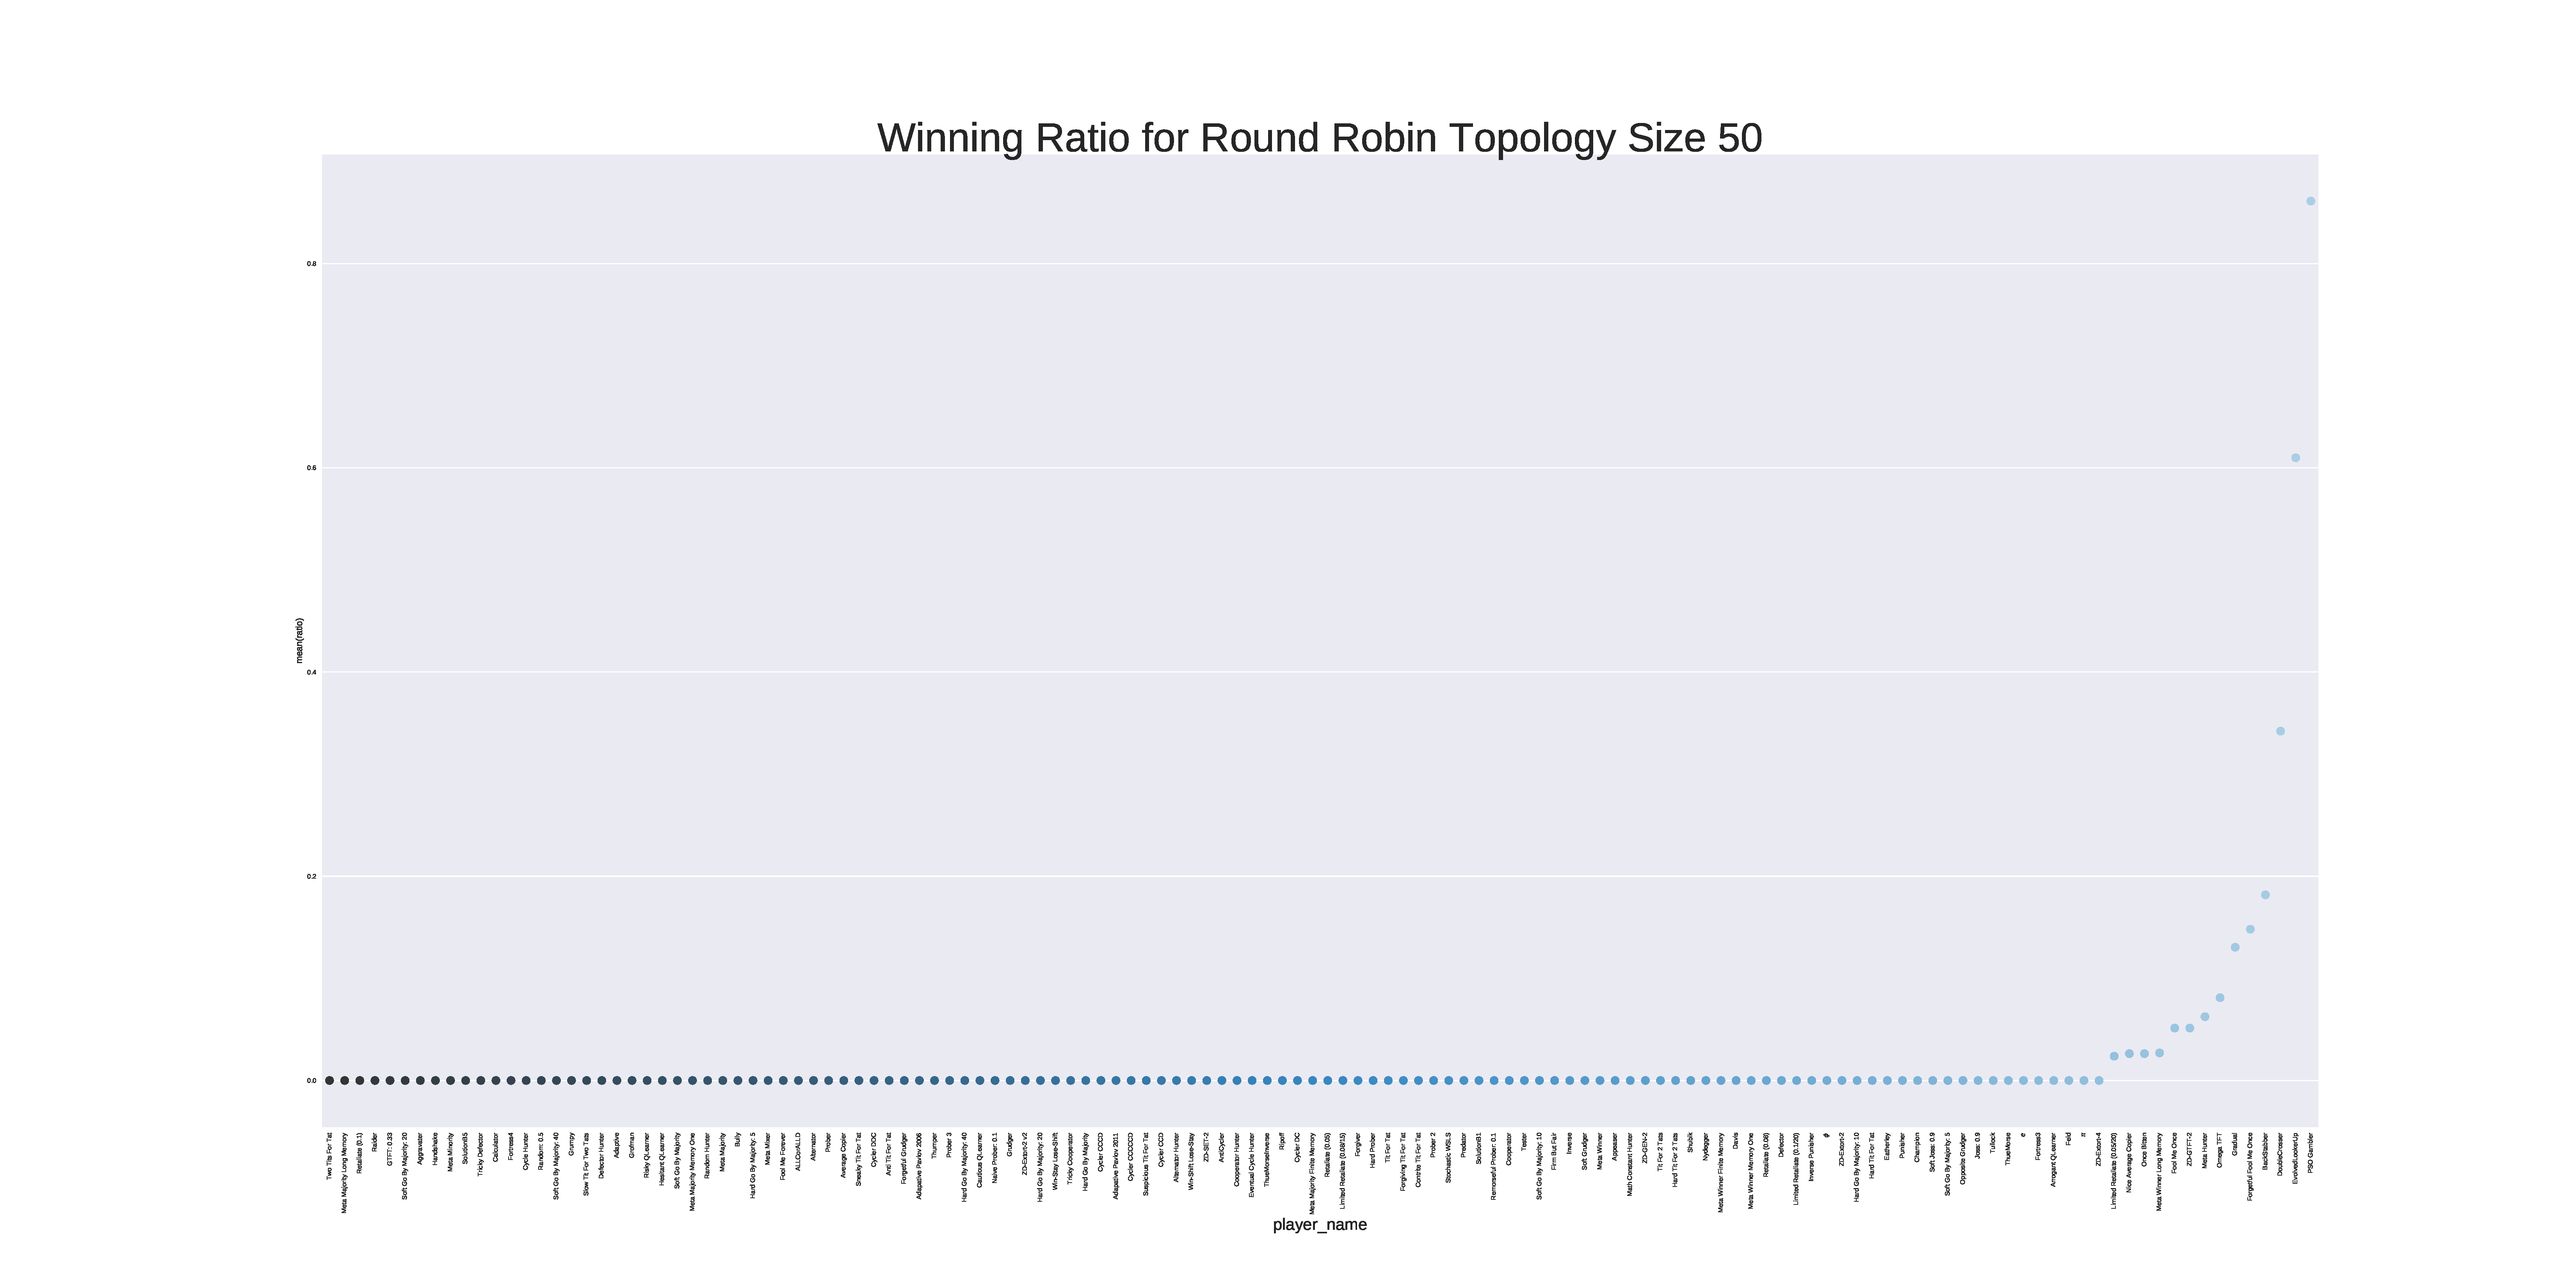
\includegraphics[width=\linewidth]{appendix/winners-Round-Robin-50.pdf}
		\caption{Winning ratio round robin topology size 50}
	\end{subfigure}
	\caption{Winning ratio for all three topologies size 50}
	\label{fig:winning-fifty}
\end{figure}

\subsection{Variation plots for normalized average score, simple networks}
\label{append:variation-plots}
In this section, as explained in \autoref{sub:normalized_av_score}, the variation of the
normalized average score has been plotted. These plots are found here.

\begin{figure}[H]
	\centering
	\begin{subfigure}[t]{0.75\textwidth}
		\centering
		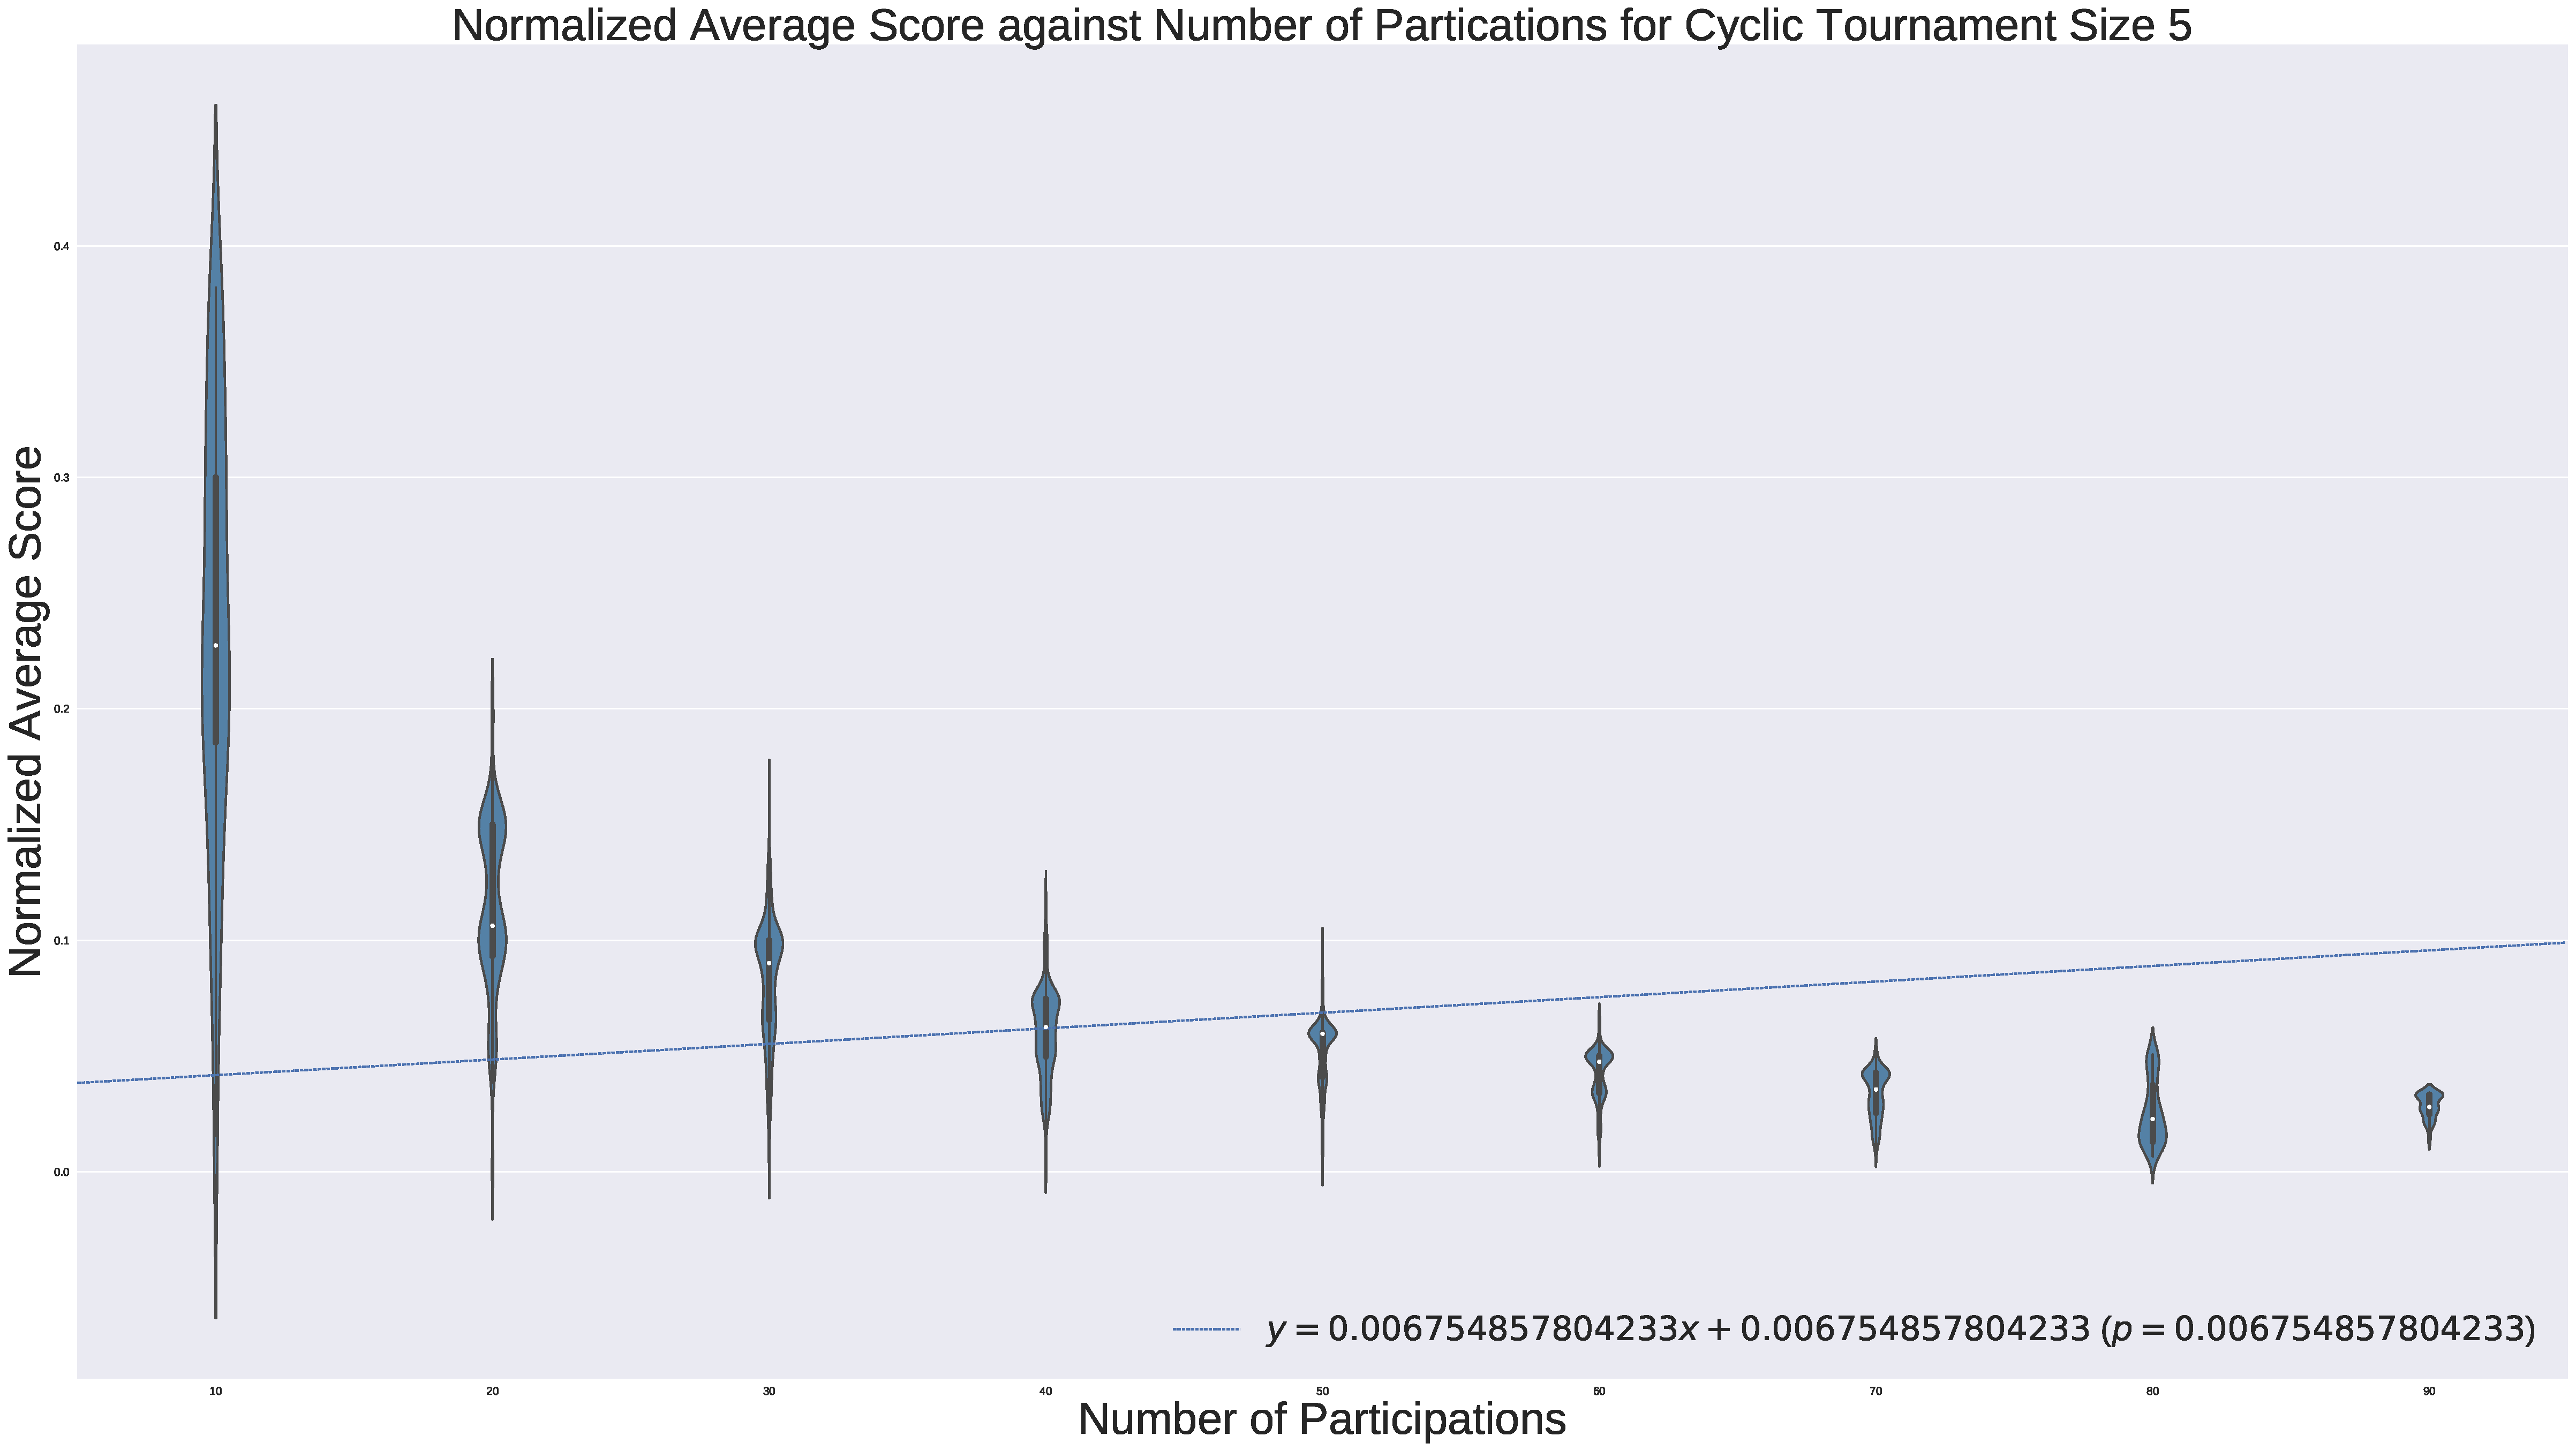
\includegraphics[width=\linewidth]{chapter-three/normalized-score-Cyclic-5.pdf}
		\caption{Normalized average score cyclic topology size 5}
	\end{subfigure}
	\hfill
	\begin{subfigure}[t]{0.75\textwidth}\centering
		\centering
		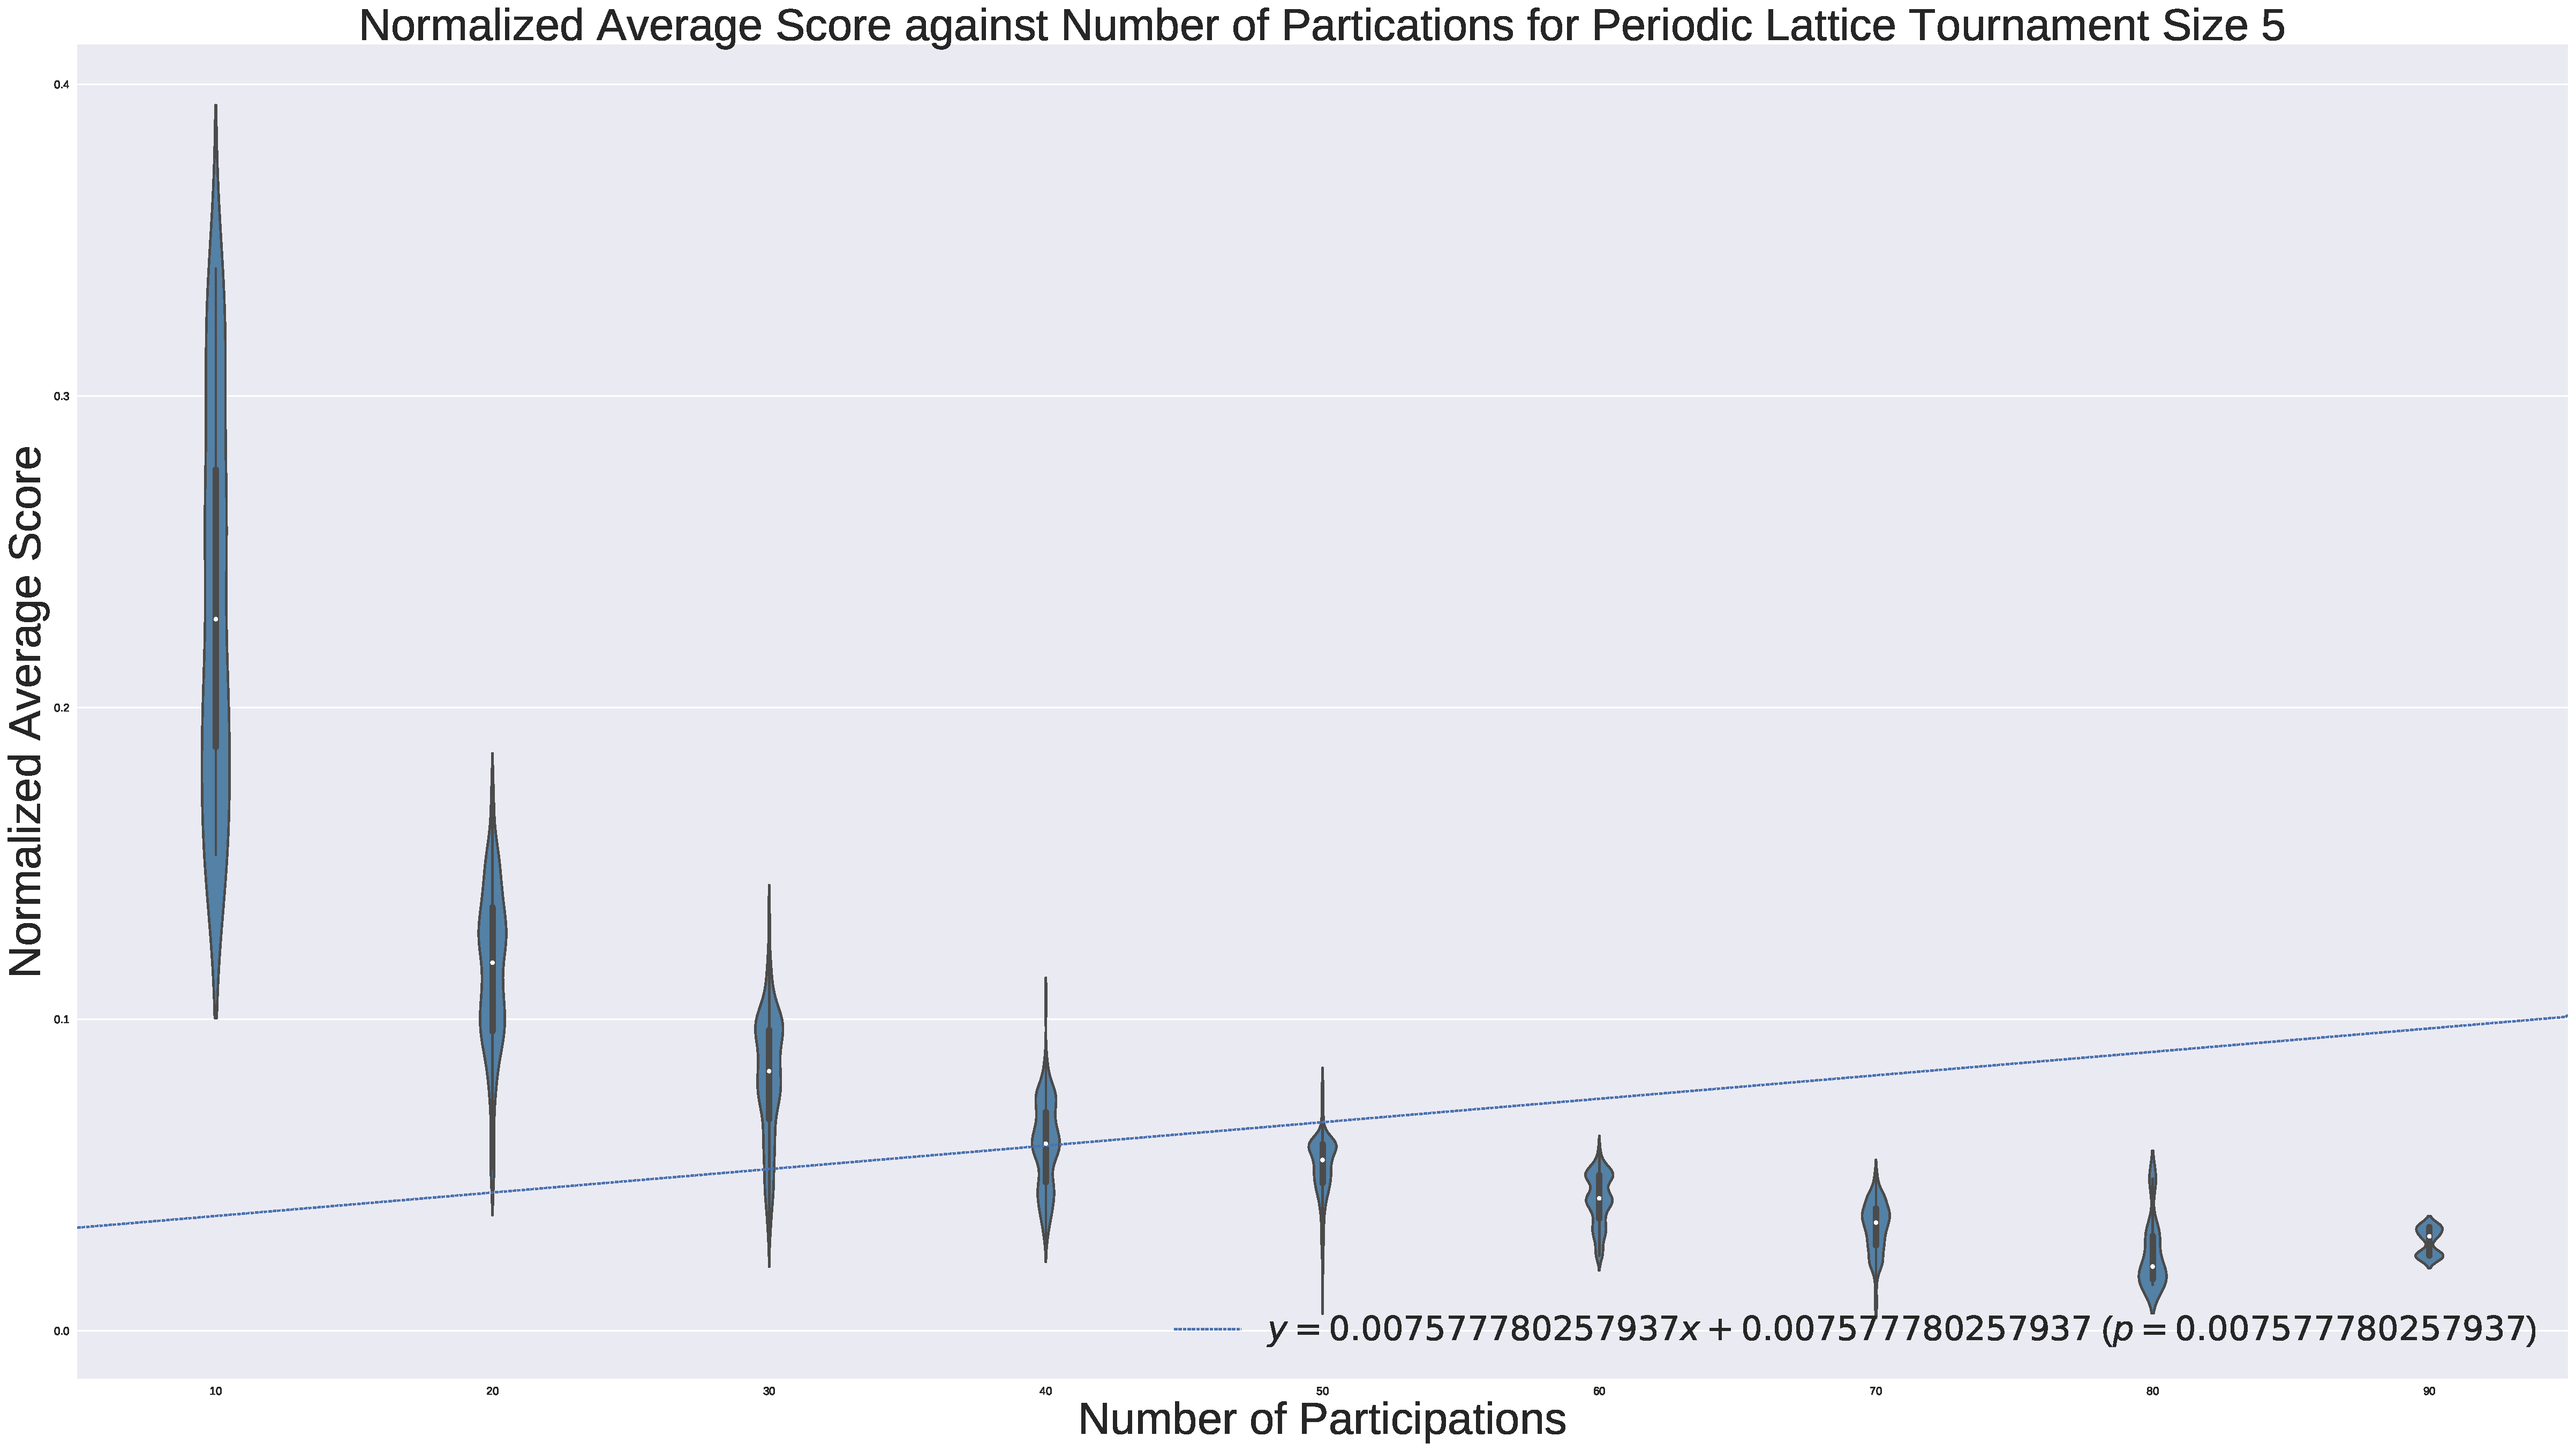
\includegraphics[width=\linewidth]{chapter-three/normalized-score-Periodic-Lattice-5.pdf}
		\caption{Normalized average score periodic lattice topology size 5}
	\end{subfigure}
	\hfill
	\begin{subfigure}[t]{0.75\textwidth}\centering
		\centering
		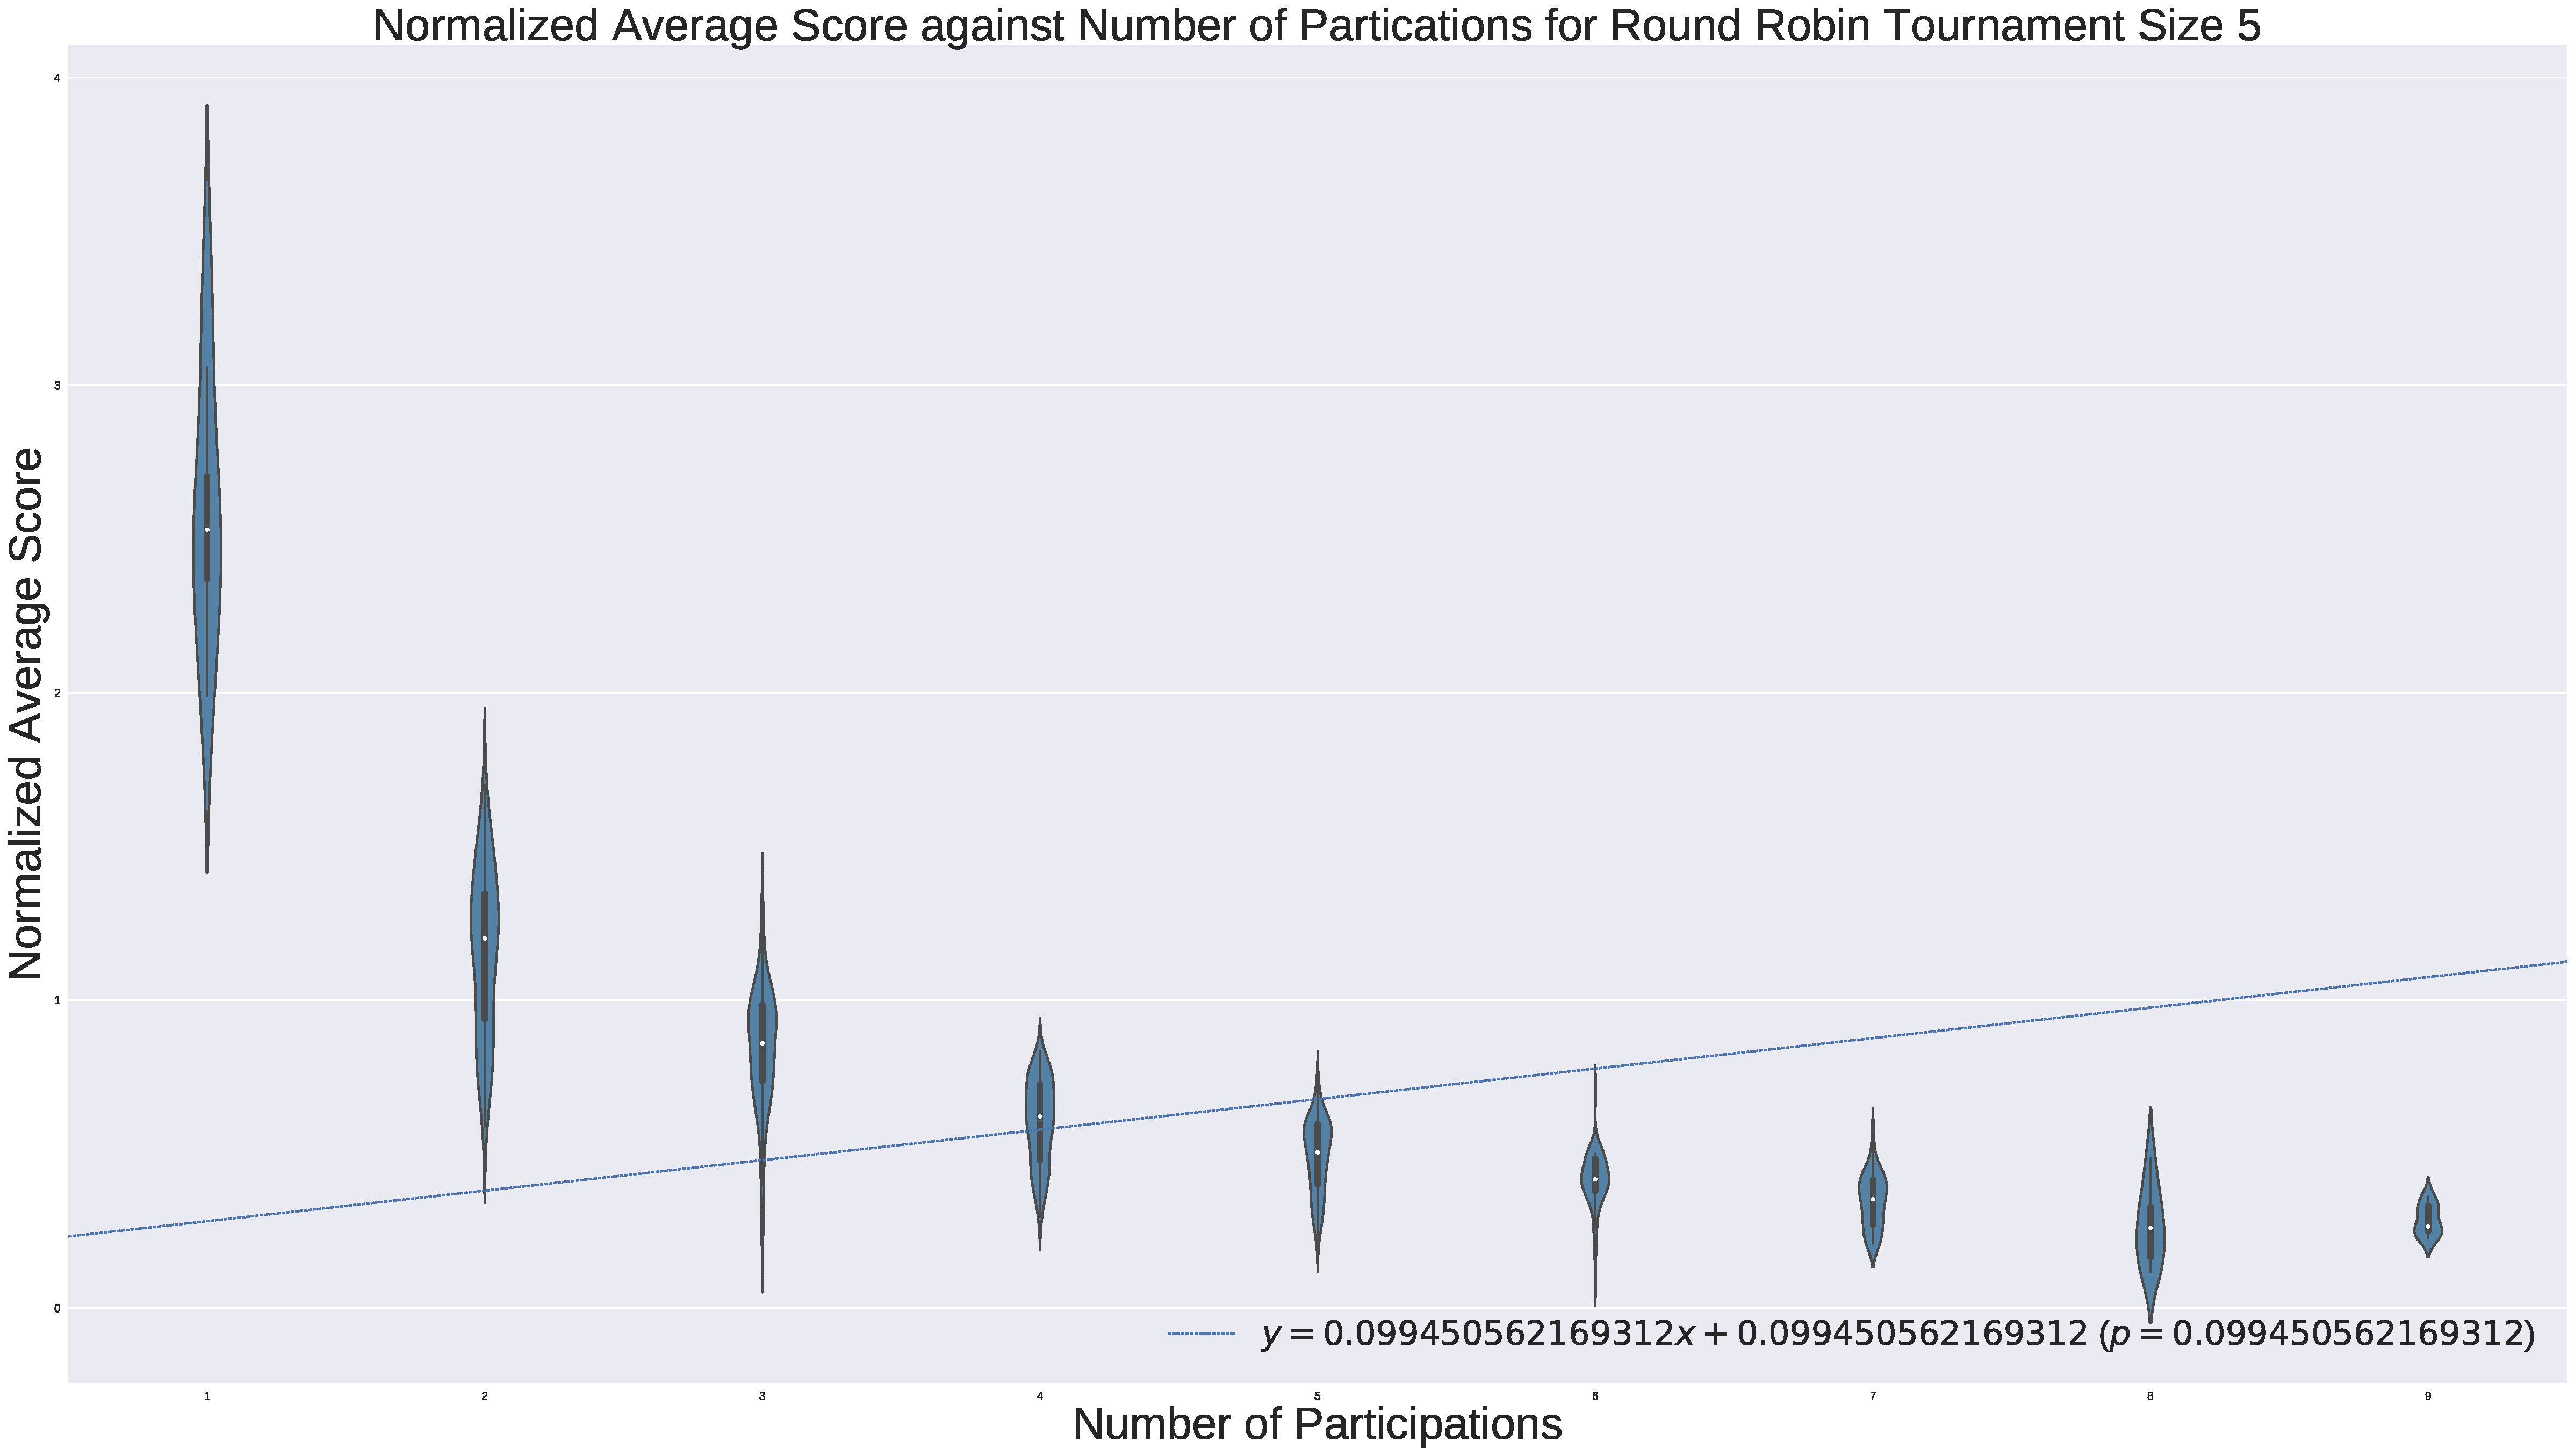
\includegraphics[width=\linewidth]{chapter-three/normalized-score-Round-Robin-5.pdf}
		\caption{Normalized average score round robin topology size 5}
	\end{subfigure}
	\caption{Normalized average score for all three topologies size 5}
	\label{fig:average-score-five}
\end{figure}

\begin{figure}[H]
	\centering
	\begin{subfigure}[t]{0.75\textwidth}
		\centering
		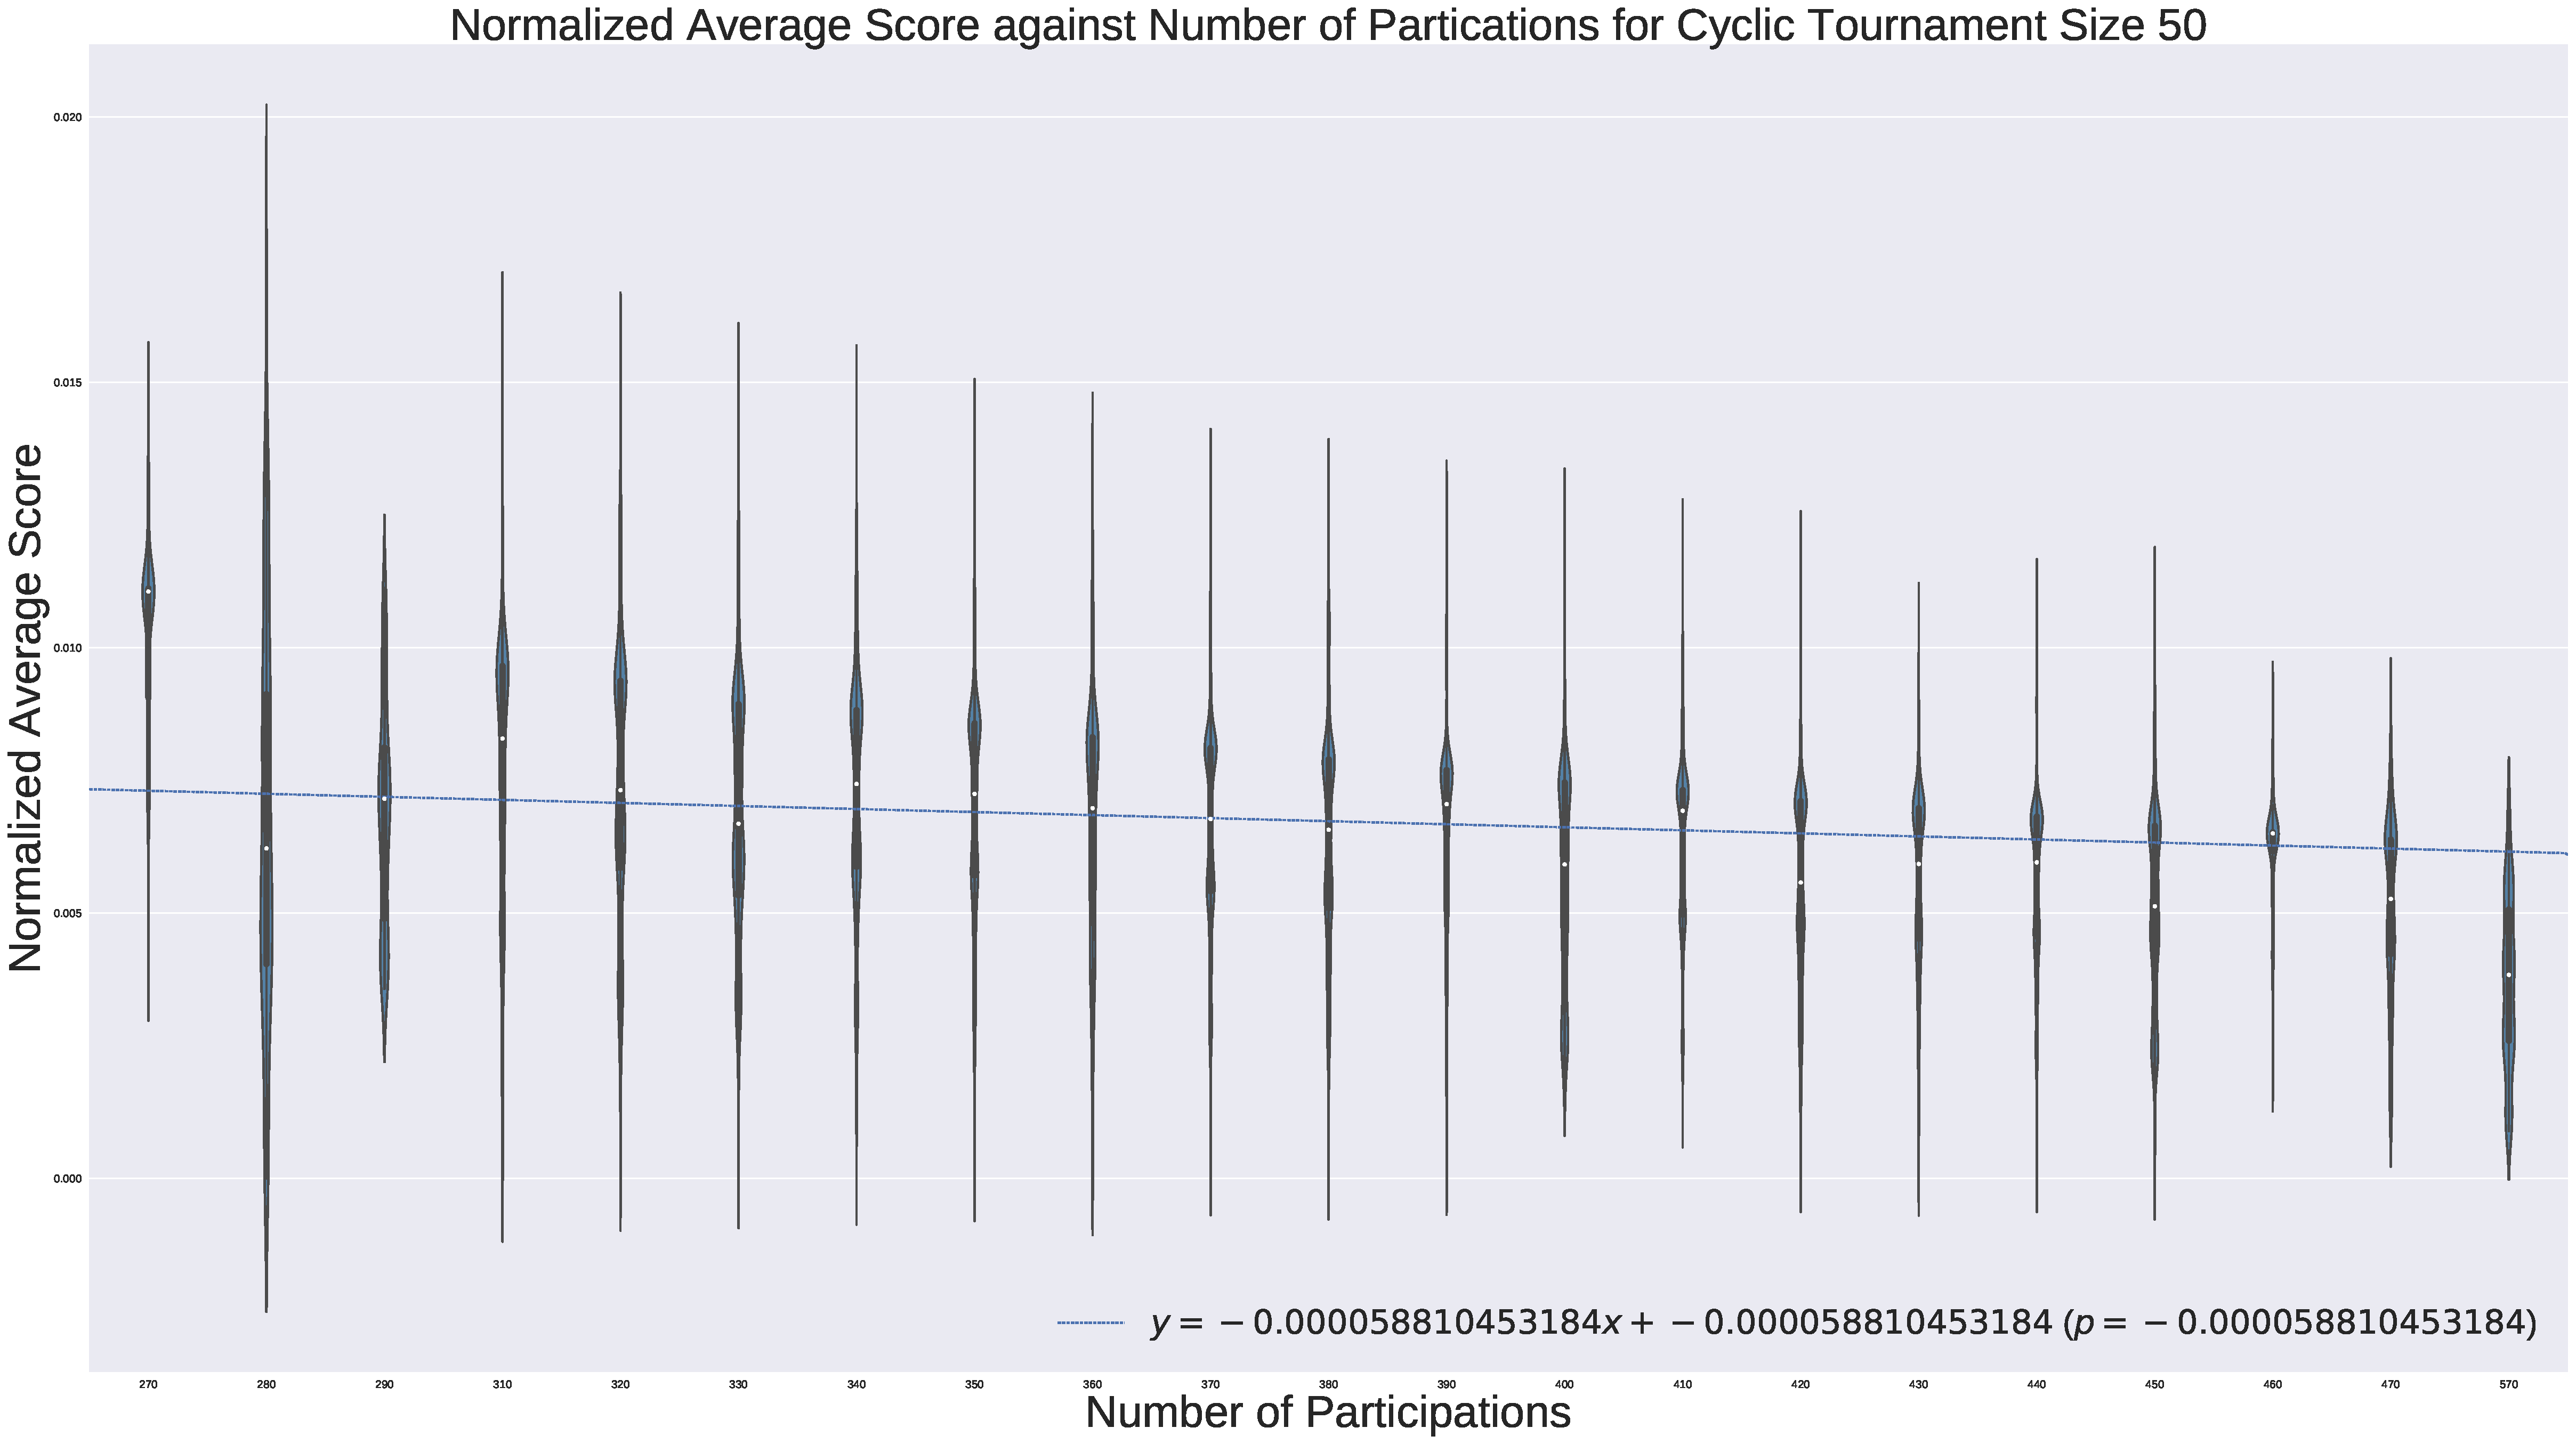
\includegraphics[width=\linewidth]{chapter-three/normalized-score-Cyclic-50.pdf}
		\caption{Normalized average score cyclic topology size 50}
	\end{subfigure}
	\hfill
	\begin{subfigure}[t]{0.75\textwidth}\centering
		\centering
		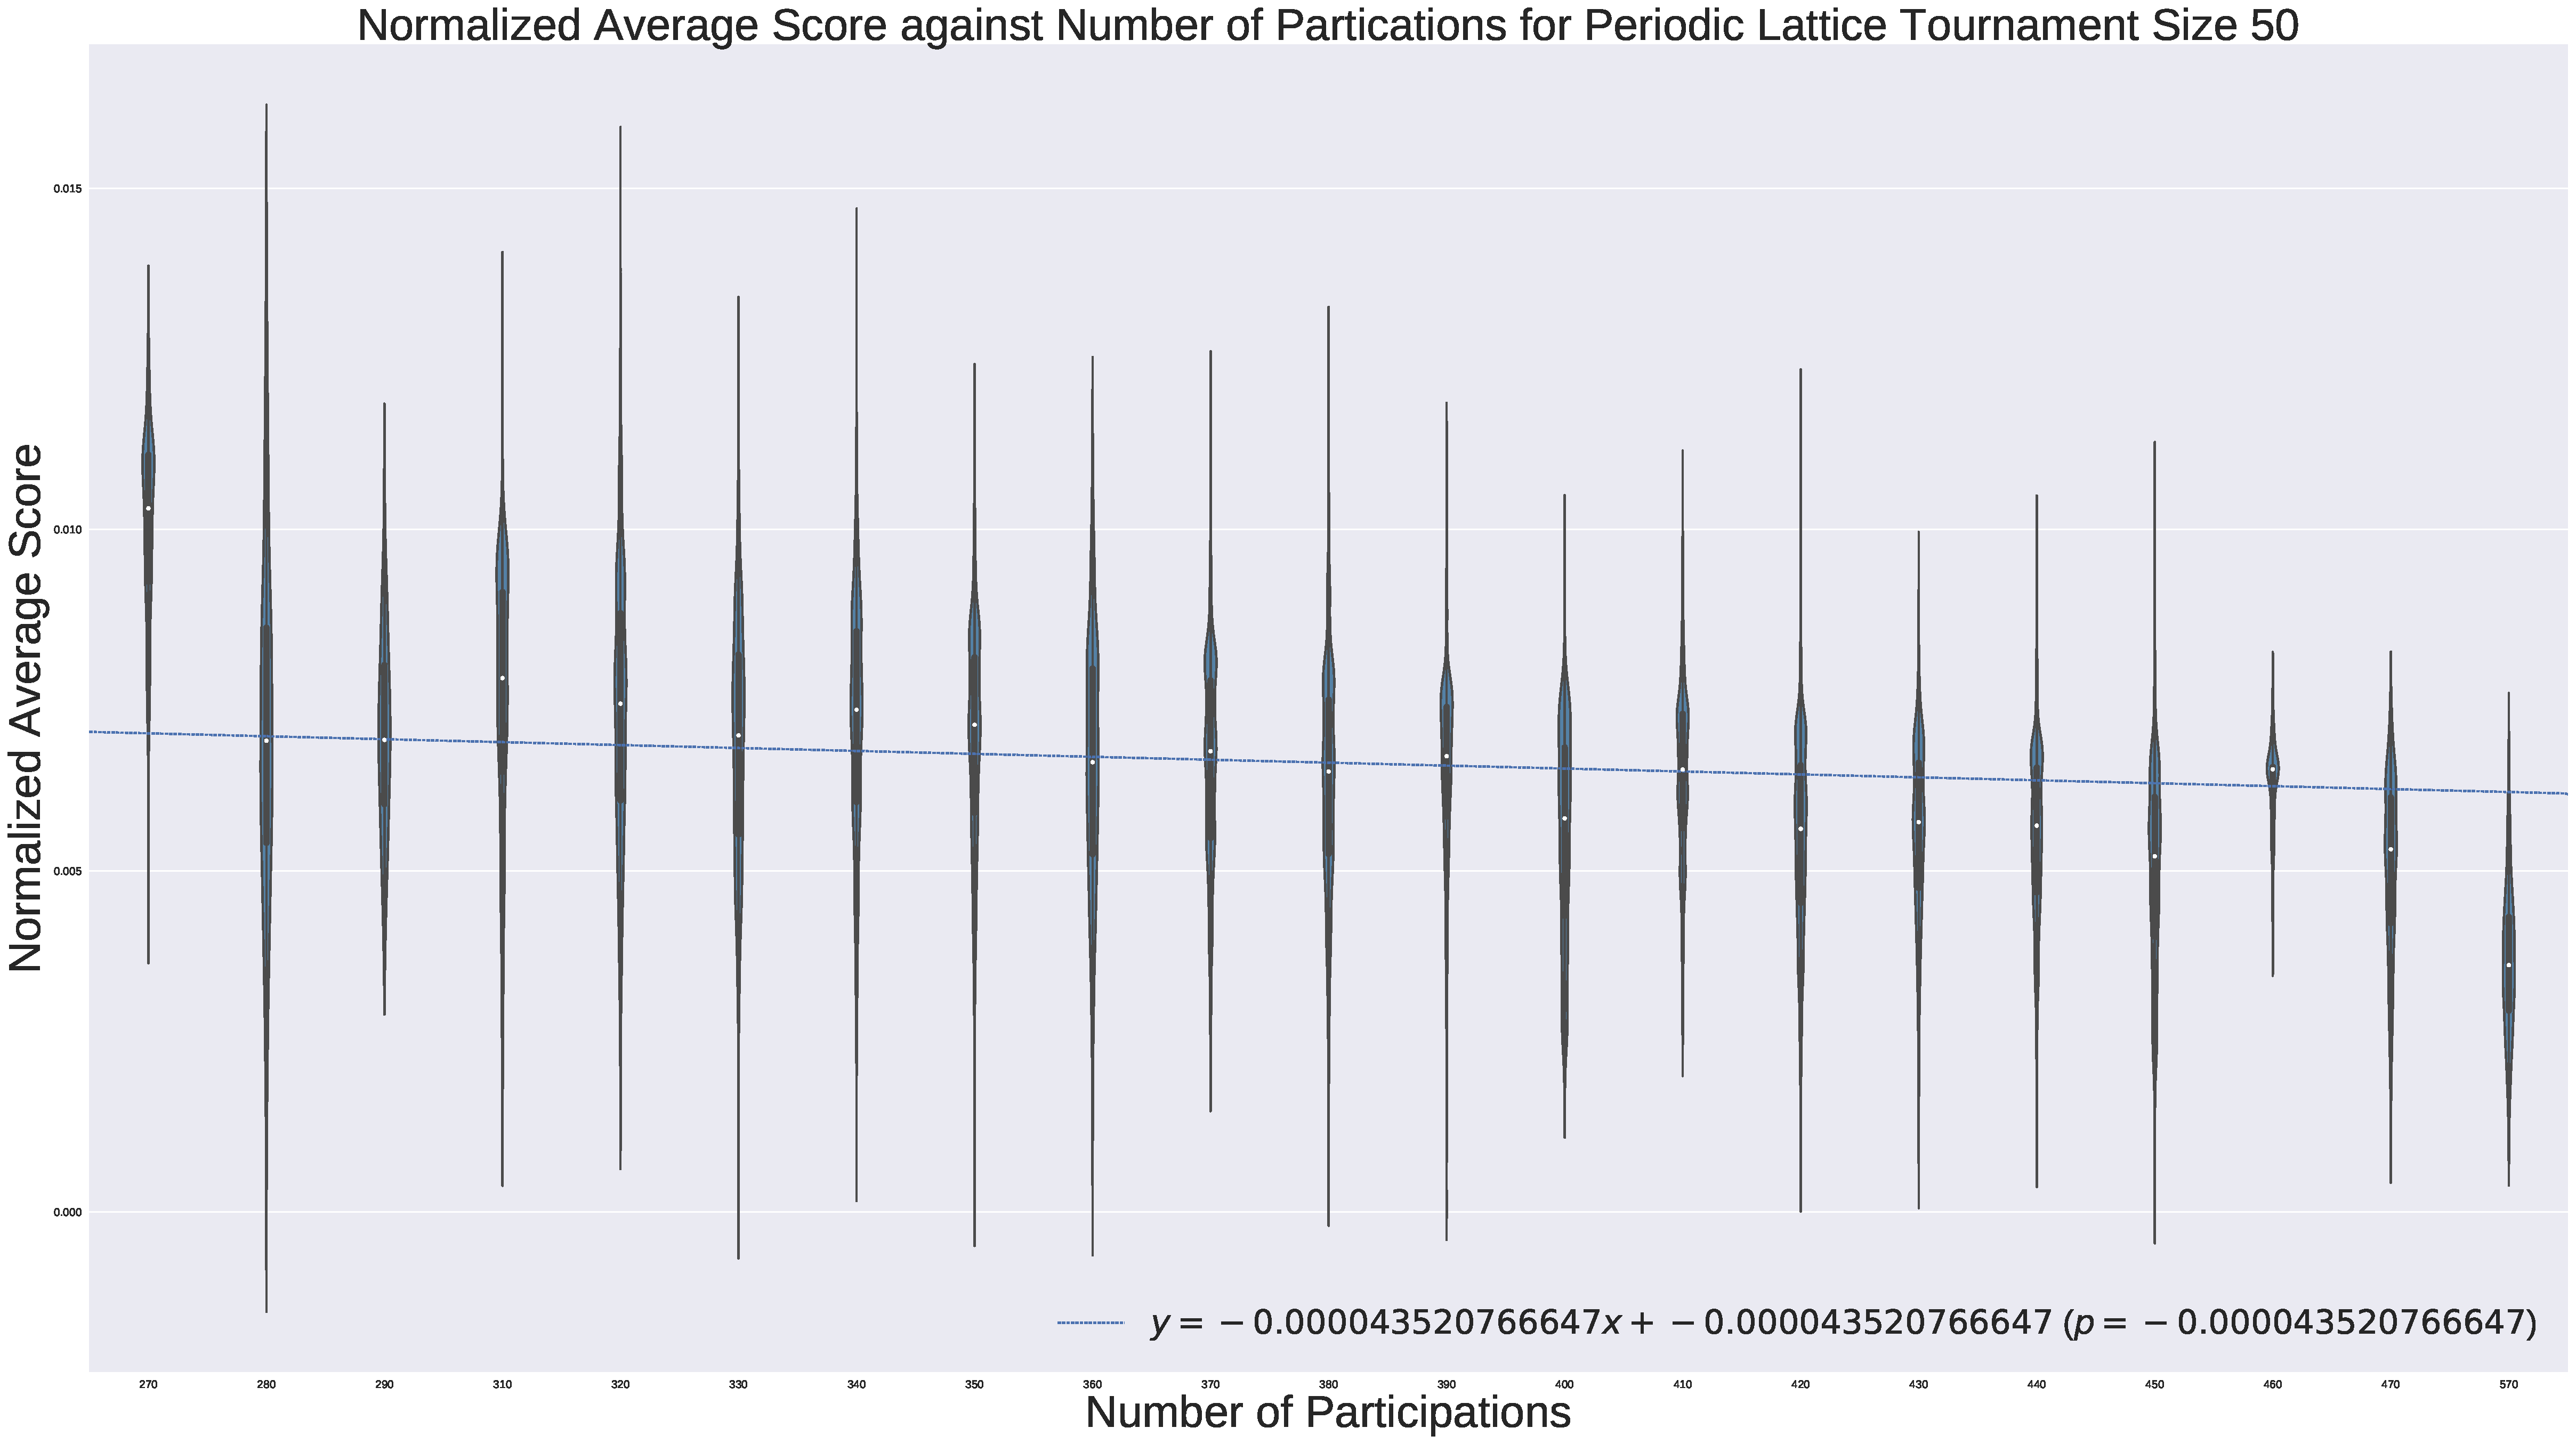
\includegraphics[width=\linewidth]{chapter-three/normalized-score-Periodic-Lattice-50.pdf}
		\caption{Normalized average score periodic lattice topology size 50}
	\end{subfigure}
	\hfill
	\begin{subfigure}[t]{0.75\textwidth}\centering
		\centering
		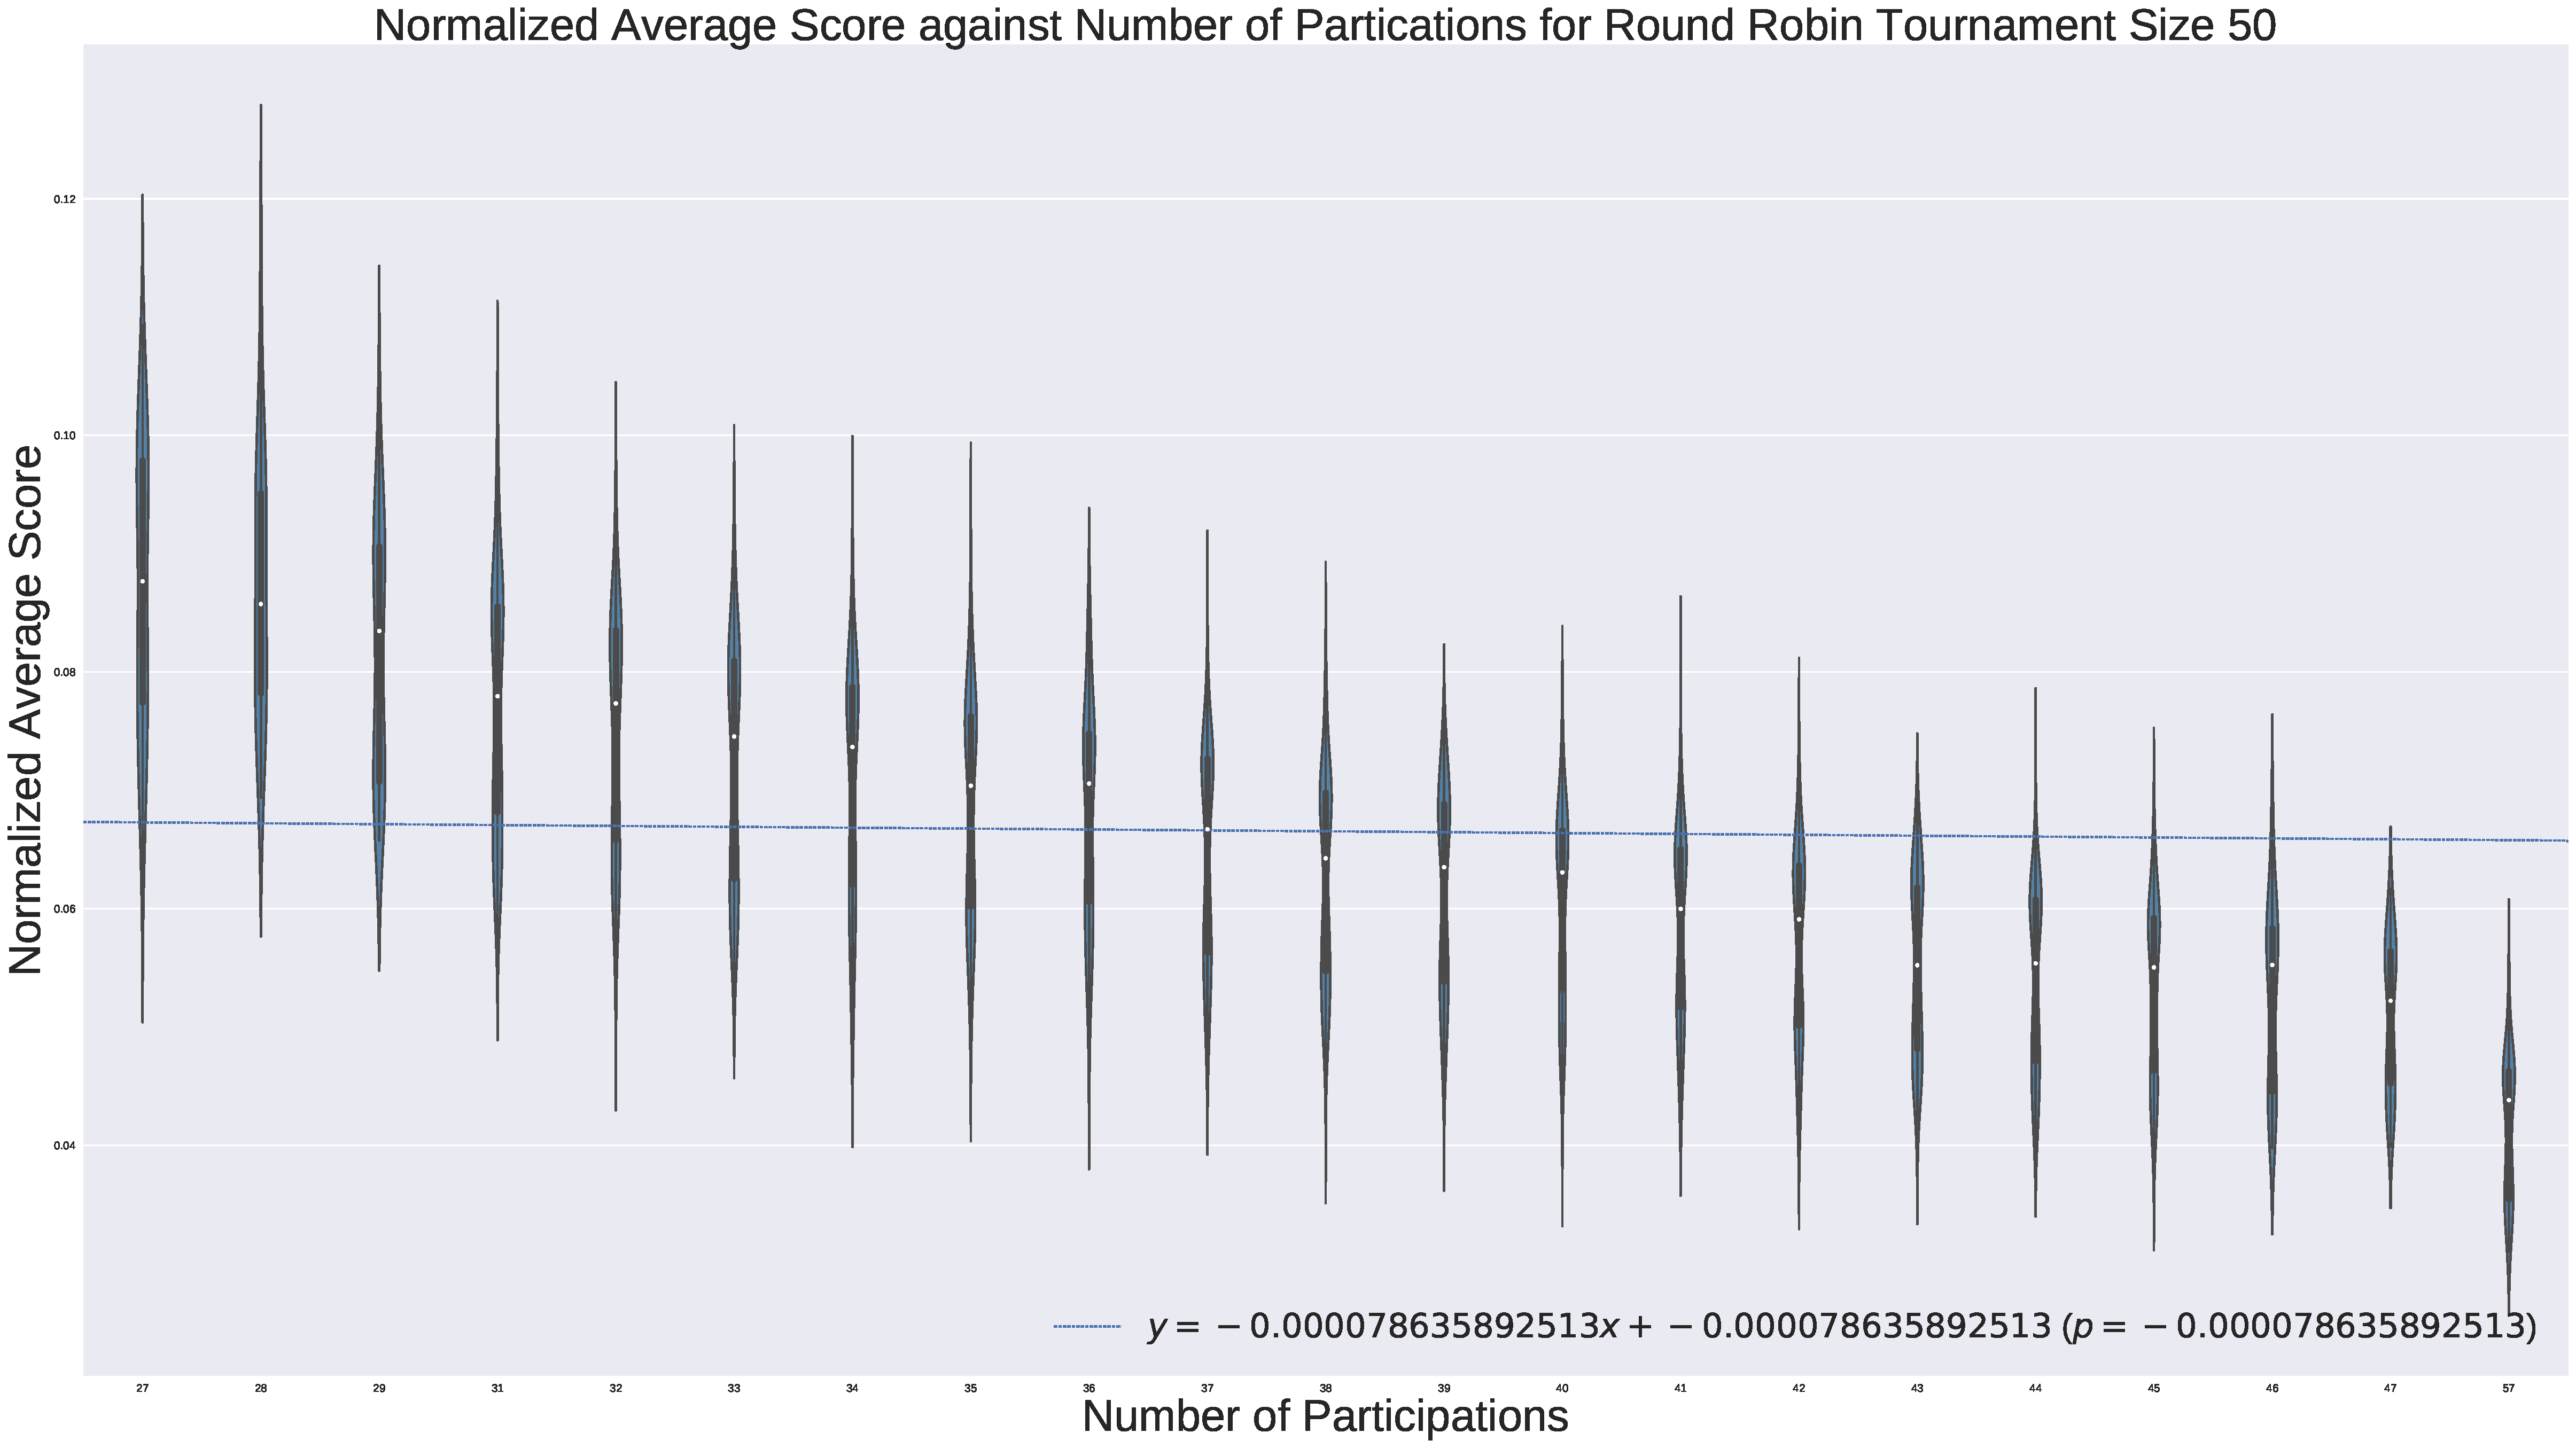
\includegraphics[width=\linewidth]{chapter-three/normalized-score-Round-Robin-50.pdf}
		\caption{Normalized average score round robin topology size 50}
	\end{subfigure}
	\caption{Normalized average score for all three topologies size 50}
	\label{fig:average-score-fifty}
\end{figure}

\section{Supplementary Tables}
\subsection{Strategies List}
\label{append:strategies}
A list of strategies and a simple explanation, on their game play.

\begin{table}[!hbtp]
	\centering
	\begin{adjustbox}{width=2\textwidth, angle=90}
		\small
		\begin{tabular}{rll}
				\toprule
	0.00   & Adaptive                    & Start with a specific sequence of C and D, then play the strategy that
	has worked best, recalculated each turn.                                                                                                                                                                                                                                                                                                                                                                                                                                                                                                                                                                                                                                                                                                                                                                                                                                                                                                      \\
	1.00   & Aggravater                  & Grudger, except that it defects on the first 3 turns                                                                              \\
	2.00   & ALLCorALLD                  & This strategy is at the parameter extreme of the ZD strategies (phi = 0).
	It simply repeats its last move, and so mimics ALLC or ALLD after round one.
	If the tournament is noisy, there will be long runs of C and D.

	For now starting choice is random of 0.6, but that was an arbitrary choice
	at implementation time.                                                                                                                                                                                                                                                                                                                                                                                                                                                                                                                                                                                                                                                                               \\
	3.00   & Alternator                  & A player who alternates between cooperating and defecting.                                                                        \\
	4.00   & Alternator Hunter           & A player who hunts for alternators.                                                                                               \\
	5.00   & AntiCycler                  & A player that follows a sequence of plays that contains no cycles:
	C CD CCD CCCD CCCCD CCCCCD ...                                                                                                                                                                                                                                                                                                                                                                                                                                                                                                                                                                                                                                                                                                                                                                                                                                                                                                                    \\
	6.00   & Anti Tit For Tat            & A strategy that plays the opposite of the opponents previous move.
	This is similar to BULLY above, except that the first move is cooperation.                                                                                                                                                                                                                                                                                                                                                                                                                                                                                                                                                                                                                                                                                                                                                                                                                                                                        \\
	7.00   & Adapative Pavlov 2006       & APavlov as defined in http://www.cs.nott.ac.uk/\textasciitilde{}pszjl/index\_files/chapter4.pdf
	(pages 10-11).

	APavlov attempts to classify its opponent as one of five strategies:
	Cooperative, ALLD, STFT, PavlovD, or Random. APavlov then responds in a
	manner intended to achieve mutual cooperation or to defect against
	uncooperative opponents.                                                                                                                                                                                                                                                                                                                                                                                                                                                                                                                                                                                                                                                              \\
	8.00   & Adapative Pavlov 2011       & APavlov as defined in http://www.graham-kendall.com/papers/lhk2011.pdf, as
	closely as can be determined.

	APavlov attempts to classify its opponent as one of four strategies:
	Cooperative, ALLD, STFT, or Random. APavlov then responds in a manner
	intended to achieve mutual cooperation or to defect against
	uncooperative opponents.                                                                                                                                                                                                                                                                                                                                                                                                                                                                                                                                                                                                                                                            \\
	9.00   & Appeaser                    & A player who tries to guess what the opponent wants.

	Switch the classifier every time the opponent plays 'D'.
	Start with 'C', switch between 'C' and 'D' when opponent plays 'D'.                                                                                                                                                                                                                                                                                                                                                                                                                                                                                                                                                                                                                                                                                                                                                                                                                               \\
	10.00  & Arrogant QLearner           & A player who learns the best strategies through the q-learning algorithm.

	This Q learner jumps to quick conclusions and care about the future.                                                                                                                                                                                                                                                                                                                                                                                                                                                                                                                                                                                                                                                                                                                                                                                                                                                                      \\
	11.00  & Average Copier              & The player will cooperate with probability p if the opponent's cooperation ratio is p.
	Starts with random decision.                                                                                                                                                                                                                                                                                                                                                                                                                                                                                                                                                                                                                                                                                                                                                                                                                                                                                                  \\
	12.00  & BackStabber                 &                                                                                                                                   \\
	13.00  & Bully                       & A player that behaves opposite to Tit For Tat, including first move.

	Starts by defecting and then does the opposite of opponent's previous move.
	This is the complete opposite of TIT FOR TAT, also called BULLY in literature.                                                                                                                                                                                                                                                                                                                                                                                                                                                                                                                                                                                                                                                                                                                                                                                 \\
	14.00  & Calculator                  & Plays like (Hard) Joss for the first 20 rounds. If periodic behavior is
	detected, defect forever. Otherwise play TFT.                                                                                                                                                                                                                                                                                                                                                                                                                                                                                                                                                                                                                                                                                                                                                                                                                                                                                                \\
	15.00  & Cautious QLearner           & A player who learns the best strategies through the q-learning algorithm.

	This Q learner is slower to come to conclusions and wants to look ahead more.                                                                                                                                                                                                                                                                                                                                                                                                                                                                                                                                                                                                                                                                                                                                                                                                                                                             \\
	16.00  & Champion                    & Strategy submitted to Axelrod's second tournament by Danny Champion.                                                              \\
	17.00  & Contrite Tit For Tat        &                                                                                                                                   \\
	18.00  & Cooperator                  & A player who only ever cooperates.                                                                                                \\
	19.00  & Cooperator Hunter           & A player who hunts for cooperators.                                                                                               \\
	20.00  & Cycle Hunter                & Hunts strategies that play cyclically, like any of the Cyclers,
	                                       Alternator, etc.                                                                                                                                                                                                                                                                                                                                                                                                                                                                                                                                                                                                                                                                                                                                                                                                                                                                                                                                     \\
	21.00  & Cycler CCCCCD               &                                                                                                                                   \\
	22.00  & Cycler CCCD                 &                                                                                                                                   \\
	23.00  & Cycler CCD                  &                                                                                                                                   \\
	24.00  & Cycler DC                   &                                                                                                                                   \\
	25.00  & Cycler DDC                  &                                                                                                                                   \\
	26.00  & Davis                       & A player starts by cooperating for 10 rounds then plays Grudger,
	defecting if at any point the opponent has defected.                                                                                                                                                                                                                                                                                                                                                                                                                                                                                                                                                                                                                                                                                                                                                                                                                                                                                                \\
	27.00  & Defector                    & A player who only ever defects.                                                                                                   \\
	28.00  & Defector Hunter             & A player who hunts for defectors.                                                                                                 \\
	29.00  & DoubleCrosser               &                                                                                                                                   \\
	30.00  & Eatherley                   & Strategy submitted to Axelrod's second tournament by Graham Eatherley.                                                            \\
	31.00  & Eventual Cycle Hunter       & Hunts strategies that eventually play cyclically                                                                                  \\
	32.00  & Feld                        & Defects when opponent defects. Cooperates with a probability that decreases
	to 0.5 at round 200.                                                                                                                                                                                                                                                                                                                                                                                                                                                                                                                                                                                                                                                                                                                                                                                                                                                                                                                     \\
	33.00  & Firm But Fair               & A Classical Strategy described in this paper (and earlier):
	http://www.math.ubc.ca/\textasciitilde{}hauert/publications/reprints/hauert\_jtb02b.pdf                                                                                                                                                                                                                                                                                                                                                                                                                                                                                                                                                                                                                                                                                                                                                                                                                                                                                   \\
	34.00  & Fool Me Forever             & Fool me once, shame on me. Teach a man to fool me and I'll be fooled for
	the rest of my life.                                                                                                                                                                                                                                                                                                                                                                                                                                                                                                                                                                                                                                                                                                                                                                                                                                                                                                                        \\
	35.00  & Fool Me Once                & Forgives one D then retaliates forever on a second D.                                                                             \\
	36.00  & Forgetful Fool Me Once      & Forgives one D then retaliates forever on a second D. Sometimes randomly
	forgets the defection count, and so keeps a secondary count separate from
	the standard count in Player.                                                                                                                                                                                                                                                                                                                                                                                                                                                                                                                                                                                                                                                                                                                                                                                                                                 \\
	37.00  & Forgetful Grudger           & A player starts by cooperating however will defect if at any point the
	opponent has defected, but forgets after mem\_length matches.                                                                                                                                                                                                                                                                                                                                                                                                                                                                                                                                                                                                                                                                                                                                                                                                                                                                                  \\
	38.00  & Forgiver                    & A player starts by cooperating however will defect if at any point
	the opponent has defected more than 10 percent of the time                                                                                                                                                                                                                                                                                                                                                                                                                                                                                                                                                                                                                                                                                                                                                                                                                                                                                        \\
	39.00  & Forgiving Tit For Tat       & A player starts by cooperating however will defect if at any point,
	the opponent has defected more than 10 percent of the time,
	and their most recent decision was defect.                                                                                                                                                                                                                                                                                                                                                                                                                                                                                                                                                                                                                                                                                                                                                                                                                                       \\
	40.00  & Fortress3                   & Finite state machine player specified in DOI:10.1109/CEC.2006.1688322.
	Note that the description in http://www.graham-kendall.com/papers/lhk2011.pdf
	is not correct.                                                                                                                                                                                                                                                                                                                                                                                                                                                                                                                                                                                                                                                                                                                                                                                                                                             \\
	41.00  & Fortress4                   & Finite state machine player specified in DOI:10.1109/CEC.2006.1688322.
	Note that the description in http://www.graham-kendall.com/papers/lhk2011.pdf
	is not correct.                                                                                                                                                                                                                                                                                                                                                                                                                                                                                                                                                                                                                                                                                                                                                                                                                                             \\
	42.00  & PSO Gambler                 & A LookerUp strategy that uses a lookup table with probability numbers
	generated using a Particle Swarm Optimisation (PSO) algorithm.

	A description of how this strategy was trained is given here:
	https://gist.github.com/GDKO/60c3d0fd423598f3c4e4                                                                                                                                                                                                                                                                                                                                                                                                                                                                                                                                                                                                                                                                                                                                                        \\
	43.00  & GTFT: 0.33                  & Generous Tit-For-Tat Strategy.                                                                                                    \\
	44.00  & Soft Go By Majority         & A player examines the history of the opponent: if the opponent has more
	defections than cooperations then the player defects.

	In case of equal
	number of defections and cooperations this player will Cooperate. Passing
	the `soft=False` keyword argument when initialising will create a
	HardGoByMajority which Defects in case of equality.

	An optional memory attribute will limit the number of turns remembered (by
	default this is 0)                                                                                                                                                                                                                                                                                                                                                                                                                                                                                                                                               \\
	45.00  & Soft Go By Majority: 10     & GoByMajority player with a memory of 10.                                                                                          \\
	46.00  & Soft Go By Majority: 20     & GoByMajority player with a memory of 20.                                                                                          \\
	47.00  & Soft Go By Majority: 40     & GoByMajority player with a memory of 40.                                                                                          \\
	48.00  & Soft Go By Majority: 5      & GoByMajority player with a memory of 5.                                                                                           \\
	49.00  & Handshake                   & Starts with C, D. If the opponent plays the same way, cooperate forever,
	else defect forever.                                                                                                                                                                                                                                                                                                                                                                                                                                                                                                                                                                                                                                                                                                                                                                                                                                                                                                                        \\
	50.00  & Hard Go By Majority         & A player examines the history of the opponent: if the opponent has more \\
	                                       defections than cooperations then the player defects. In case of equal \\
	                                       number of defections and cooperations this player will Defect. \\
	                                      An optional memory attribute will limit the number of turns remembered (by \\
	                                      default this is 0)                                                                                                                                                                                                                                                                                                                                                                                                                                                                                                                                                                                                                                                                                             \\
	51.00  & Hard Go By Majority: 10     & HardGoByMajority player with a memory of 10.                                                                                      \\
	52.00  & Hard Go By Majority: 20     & HardGoByMajority player with a memory of 20.                                                                                      \\
	53.00  & Hard Go By Majority: 40     & HardGoByMajority player with a memory of 40.                                                                                      \\
	54.00  & Hard Go By Majority: 5      & HardGoByMajority player with a memory of 5.                                                                                       \\
	55.00  & \$\textbackslash{}phi\$     & The player will always aim to bring the ratio of co-operations to defections closer to the golden mean                            \\
	56.00  & Gradual                     & A player that punishes defections with a growing number of defections
	but after punishing enters a calming state and cooperates no matter what
	the opponent does for two rounds.

	http://perso.uclouvain.be/vincent.blondel/workshops/2003/beaufils.pdf                                                                                                                                                                                                                                                                                                                                                                                                                                                                                                                                                                                                                                                                                                                                                      \\
	57.00  & Grofman                     & Cooperate on the first 2 moves. Return opponent's move for the next 5.
	Then cooperate if the last round's moves were the same, otherwise cooperate
	with probability 2/7.                                                                                                                                                                                                                                                                                                                                                                                                                                                                                                                                                                                                                                                                                                                                                                                                                                         \\
	58.00  & Grudger                     & A player starts by cooperating however will defect if at any point the opponent has defected.                                     \\
	59.00  & Grumpy                      & A player that defects after a certain level of grumpiness.
	Grumpiness increases when the opponent defects and decreases
	when the opponent co-operates.                                                                                                                                                                                                                                                                                                                                                                                                                                                                                                                                                                                                                                                                                                                                                                                                                                                           \\
	60.00  & Hard Prober                 & Plays D, D, C, C initially. Defects forever if opponent cooperated in moves
	2 and 3. Otherwise plays TFT.                                                                                                                                                                                                                                                                                                                                                                                                                                                                                                                                                                                                                                                                                                                                                                                                                                                                                                            \\
	61.00  & Hard Tit For 2 Tats         & A variant of Tit For Two Tats that uses a longer history for
	retaliation.                                                                                                                                                                                                                                                                                                                                                                                                                                                                                                                                                                                                                                                                                                                                                                                                                                                                                                                                            \\
	62.00  & Hard Tit For Tat            & A variant of Tit For Tat that uses a longer history for retaliation.                                                              \\
	63.00  & Hesitant QLearner           & A player who learns the best strategies through the q-learning algorithm.

	This Q learner is slower to come to conclusions and does not look ahead much.                                                                                                                                                                                                                                                                                                                                                                                                                                                                                                                                                                                                                                                                                                                                                                                                                                                             \\
	64.00  & Inverse                     & A player who defects with a probability that diminishes relative to how
	long ago the opponent defected.                                                                                                                                                                                                                                                                                                                                                                                                                                                                                                                                                                                                                                                                                                                                                                                                                                                                                                              \\
	65.00  & Inverse Punisher            & A player starts by cooperating however will defect if at any point the
	opponent has defected, but forgets after mem\_length matches, with
	1 \ensuremath{<}= mem\_length \ensuremath{<}= 20 proportional to the amount of time the opponent
	has played C. The inverse of Punisher.                                                                                                                                                                                                                                                                                                                                                                                                                                                                                                                                                                                                                                                                                                                                                        \\
	66.00  & Joss: 0.9                   & Cooperates with probability 0.9 when the opponent cooperates, otherwise
	emulates Tit-For-Tat.                                                                                                                                                                                                                                                                                                                                                                                                                                                                                                                                                                                                                                                                                                                                                                                                                                                                                                                        \\
	67.00  & Limited Retaliate (0.1/20)  & A player that co-operates unless the opponent defects and wins.
	It will then retaliate by defecting. It stops when either, it has beaten
	the opponent 10 times more often that it has lost or it reaches the
	retaliation limit (20 defections).                                                                                                                                                                                                                                                                                                                                                                                                                                                                                                                                                                                                                                                                                                                                                              \\
	68.00  & Limited Retaliate (0.08/15) & LimitedRetaliate player with a threshold of 8 percent and a
	retaliation limit of 15.                                                                                                                                                                                                                                                                                                                                                                                                                                                                                                                                                                                                                                                                                                                                                                                                                                                                                                                                 \\
	69.00  & Limited Retaliate (0.05/20) & LimitedRetaliate player with a threshold of 5 percent and a
	retaliation limit of 20.                                                                                                                                                                                                                                                                                                                                                                                                                                                                                                                                                                                                                                                                                                                                                                                                                                                                                                                                 \\
	70.00  & EvolvedLookerUp             & A LookerUp strategy that uses a lookup table generated using an evolutionary
	algorithm.

	A description of how this strategy was trained is given here:
	http://mojones.net/evolving-strategies-for-an-iterated-prisoners-dilemma-tournament.html                                                                                                                                                                                                                                                                                                                                                                                                                                                                                                                                                                                                                                                                                                                                                              \\
	71.00  & Math Constant Hunter        & A player who hunts for mathematical constant players.                                                                             \\
	72.00  & Naive Prober: 0.1           & Like tit-for-tat, but it occasionally defects with a small probability.

	For reference see: "Engineering Design of Strategies for Winning
	Iterated Prisoner's Dilemma Competitions" by Jiawei Li, Philip Hingston,
	and Graham Kendall.  IEEE TRANSACTIONS ON COMPUTATIONAL INTELLIGENCE AND AI
	IN GAMES, VOL. 3, NO. 4, DECEMBER 2011                                                                                                                                                                                                                                                                                                                                                                                                                                                                                                                                                                                                                                                                    \\
	73.00  & Nice Average Copier         & Same as Average Copier, but always starts by cooperating.                                                                         \\
	74.00  & Nydegger                    & The program begins with tit for tat for the first three moves, except that
                                        	if it was the only one to cooperate on the first move and the only one to
                                        	defect on the second move, it defects on the third move. After the third move,
                                        	its choice is determined from the 3 preceding outcomes in the following manner.
                                        	Let A be the sum formed by counting the other's defection as 2 points and one's
                                        	own as 1 point, and giving weights of 16, 4, and 1 to the preceding three
                                        	moves in chronological order. The choice can be described as defecting only
                                        	when A equals 1, 6, 7, 17, 22, 23, 26, 29, 30, 31, 33, 38, 39, 45, 49, 54,
                                        	55, 58, or 61. Thus if all three preceding moves are mutual defection,
                                        	A = 63 and the rule cooperates. This rule was designed for use in laboratory
                                        	experiments as a stooge which had a memory and appeared to be trustworthy,
                                        	potentially cooperative, but not gullible.

	-- Axelrod, "Effective Choice in the Prisoner's Dilemma" \\
	75.00  & Omega TFT                   & OmegaTFT modifies TFT in two ways:
	-- checks for deadlock loops of alternating rounds of (C, D) and (D, C),
	and attempting to break them
	-- uses a more sophisticated retaliation mechanism that is noise tolerant.                                                                                                                                                                                                                                                                                                                                                                                                                                                                                                                                                                                                                                                                                                                                                                                 \\
	76.00  & Once Bitten                 & Cooperates once when the opponent defects, but if they defect twice in a row defaults to forgetful grudger for 10 turns defecting \\
	77.00  & Opposite Grudger            & A player starts by defecting however will cooperate if at any point the opponent has cooperated.                                  \\
	78.00  & \$\textbackslash{}pi\$      & The player will always aim to bring the ratio of co-operations to defections closer to the pi                                     \\
	79.00  & Predator                    & Finite state machine player specified in DOI:10.1109/CEC.2006.1688322.                                                            \\
	80.00  & Prober                      & Plays D, C, C initially. Defects forever if opponent cooperated in moves 2
	and 3. Otherwise plays TFT.                                                                                                                                                                                                                                                                                                                                                                                                                                                                                                                                                                                                                                                                                                                                                                                                                                                                                                               \\
	81.00  & Prober 2                    & Plays D, C, C initially. Cooperates forever if opponent played D then C
	in moves 2 and 3. Otherwise plays TFT.                                                                                                                                                                                                                                                                                                                                                                                                                                                                                                                                                                                                                                                                                                                                                                                                                                                                                                       \\
	82.00  & Prober 3                    & Plays D, C initially. Defects forever if opponent played C in moves 2.
	Otherwise plays TFT.                                                                                                                                                                                                                                                                                                                                                                                                                                                                                                                                                                                                                                                                                                                                                                                                                                                                                                                          \\
	83.00  & Punisher                    & A player starts by cooperating however will defect if at any point the
	opponent has defected, but forgets after meme\_length matches, with
	1\ensuremath{<}=mem\_length\ensuremath{<}=20 proportional to the amount of time the opponent has
	played D, punishing that player for playing D too often.                                                                                                                                                                                                                                                                                                                                                                                                                                                                                                                                                                                                                                                                                                                                     \\
	84.00  & Raider                      & FSM player described in DOI:10.1109/FOCI.2014.7007818                                                                             \\
	85.00  & Random: 0.5                 & A player who randomly chooses between cooperating and defecting.                                                                  \\
	86.00  & Random Hunter               & A player who hunts for random players.                                                                                            \\
	87.00  & Remorseful Prober: 0.1      & Like Naive Prober, but it remembers if the opponent responds to a random
	defection with a defection by being remorseful and cooperating.

	For reference see: "Engineering Design of Strategies for Winning
	Iterated Prisoner's Dilemma Competitions" by Jiawei Li, Philip Hingston,
	and Graham Kendall.  IEEE TRANSACTIONS ON COMPUTATIONAL INTELLIGENCE AND AI
	IN GAMES, VOL. 3, NO. 4, DECEMBER 2011

	A more complete description is given in "The Selfish Gene"
	(https://books.google.co.uk/books?id=ekonDAAAQBAJ):

	"Remorseful Prober remembers whether it has just spontaneously defected, and
	whether the result was prompt retaliation. If so, it 'remorsefully' allows
	its opponent 'one free hit' without retaliating."                                                                                                                                                                                                                                                \\
	88.00  & Retaliate (0.1)             & A player starts by cooperating but will retaliate once the opponent
	has won more than 10 percent times the number of defections the player has.                                                                                                                                                                                                                                                                                                                                                                                                                                                                                                                                                                                                                                                                                                                                                                                                                                                                      \\
	89.00  & Retaliate (0.08)            & Retaliate player with a threshold of 8 percent.                                                                                   \\
	90.00  & Retaliate (0.05)            & Retaliate player with a threshold of 5 percent.                                                                                   \\
	91.00  & Ripoff                      & FSM player described in DOI:10.1109/TEVC.2008.920675.                                                                             \\
	92.00  & Risky QLearner              & A player who learns the best strategies through the q-learning algorithm.

	This qlearner is quick to come to conclusions and doesn't care about the future.                                                                                                                                                                                                                                                                                                                                                                                                                                                                                                                                                                                                                                                                                                                                                                                                                                                          \\
	93.00  & Shubik                      & Plays like Tit-For-Tat with the following modification. After
	each retaliation, the number of rounds that Shubik retaliates
	increases by 1.                                                                                                                                                                                                                                                                                                                                                                                                                                                                                                                                                                                                                                                                                                                                                                                                                                                                      \\
	94.00  & Slow Tit For Two Tats       & A player plays C twice, then if the opponent plays the same move twice,
	plays that move                                                                                                                                                                                                                                                                                                                                                                                                                                                                                                                                                                                                                                                                                                                                                                                                                                                                                                                             \\
	95.00  & Sneaky Tit For Tat          & Tries defecting once and repents if punished.                                                                                     \\
	96.00  & Soft Grudger                & A modification of the Grudger strategy. Instead of punishing by always
	defecting: punishes by playing: D, D, D, D, C, C. (Will continue to
	cooperate afterwards).

	For reference see: "Engineering Design of Strategies for Winning
	Iterated Prisoner's Dilemma Competitions" by Jiawei Li, Philip Hingston,
	and Graham Kendall.  IEEE TRANSACTIONS ON COMPUTATIONAL INTELLIGENCE AND AI
	IN GAMES, VOL. 3, NO. 4, DECEMBER 2011                                                                                                                                                                                                                                                                                                                                                                                                                                                                                                                                                                  \\
	97.00  & Soft Joss: 0.9              & Defects with probability 0.9 when the opponent defects, otherwise
	emulates Tit-For-Tat.                                                                                                                                                                                                                                                                                                                                                                                                                                                                                                                                                                                                                                                                                                                                                                                                                                                                                                                              \\
	98.00  & SolutionB1                  & FSM player described in DOI:10.1109/TCIAIG.2014.2326012.                                                                          \\
	99.00  & SolutionB5                  & FSM player described in DOI:10.1109/TCIAIG.2014.2326012.                                                                          \\
	100.00 & Stochastic WSLS             & Stochastic WSLS, similar to Generous TFT                                                                                          \\
	101.00 & Suspicious Tit For Tat      & A TFT that initially defects.                                                                                                     \\
	102.00 & Tester                      & Submitted to Axelrod's second tournament by David Gladstein.

	Defects on the first move and plays TFT if the opponent ever defects (after
	one apology cooperation round). Otherwise alternate cooperation and defection.                                                                                                                                                                                                                                                                                                                                                                                                                                                                                                                                                                                                                                                                                                                                                                                         \\
	103.00 & ThueMorse                   & A player who cooperates or defects according to the Thue-Morse sequence.

	The first few terms of the Thue-Morse sequence are:
	0 1 1 0 1 0 0 1 1 0 0 1 0 1 1 0 . . .                                                                                                                                                                                                                                                                                                                                                                                                                                                                                                                                                                                                                                                                                                                                                                                                                                              \\
	104.00 & ThueMorseInverse            & A player who defects or cooperates according to the Thue-Morse sequence
	(Inverse of ThueMorse).                                                                                                                                                                                                                                                                                                                                                                                                                                                                                                                                                                                                                                                                                                                                                                                                                                                                                                                      \\
	105.00 & Thumper                     & FSM player described in DOI:10.1109/TEVC.2008.920675.                                                                             \\
	106.00 & Tit For Tat                 & A player starts by cooperating and then mimics the previous action of the
	opponent.

	Note that the code for this strategy is written in a fairly verbose
	way. This is done so that it can serve as an example strategy for
	those who might be new to Python.                                                                                                                                                                                                                                                                                                                                                                                                                                                                                                                                                                                                                                                                                                                                             \\
	107.00 & Tit For 2 Tats              & A player starts by cooperating and then defects only after two defects by opponent.                                               \\
	108.00 & Tricky Cooperator           & A cooperator that is trying to be tricky.                                                                                         \\
	109.00 & Tricky Defector             & A defector that is trying to be tricky.                                                                                           \\
	110.00 & Tullock                     & Cooperates for the first 11 rounds then randomly cooperates 10\% less often
	than the opponent has in previous rounds.                                                                                                                                                                                                                                                                                                                                                                                                                                                                                                                                                                                                                                                                                                                                                                                                                                                                                                 \\
	111.00 & Two Tits For Tat            & A player starts by cooperating and replies to each defect by two defections.                                                      \\
	112.00 & Win-Shift Lose-Stay         & Win-Shift Lose-Stay, also called Reverse Pavlov.

	For reference see: "Engineering Design of Strategies for Winning
	Iterated Prisoner's Dilemma Competitions" by Jiawei Li, Philip Hingston,
	and Graham Kendall.  IEEE TRANSACTIONS ON COMPUTATIONAL INTELLIGENCE AND AI
	IN GAMES, VOL. 3, NO. 4, DECEMBER 2011                                                                                                                                                                                                                                                                                                                                                                                                                                                                                                                                                                                                                                                                                           \\
	113.00 & Win-Stay Lose-Shift         & Win-Stay Lose-Shift, also called Pavlov.                                                                                          \\
	114.00 & ZD-Extort-2                 & An Extortionate Zero Determinant Strategy with l=P.                                                                               \\
	115.00 & ZD-Extort-2 v2              & An Extortionate Zero Determinant Strategy with l=1.                                                                               \\
	116.00 & ZD-Extort-4                 & An Extortionate Zero Determinant Strategy with l=1, s=1/4. TFT is the
	other extreme (with l=3, s=1)                                                                                                                                                                                                                                                                                                                                                                                                                                                                                                                                                                                                                                                                                                                                                                                                                                                                                                                  \\
	117.00 & ZD-GTFT-2                   & A Generous Zero Determinant Strategy with l=R.                                                                                    \\
	118.00 & ZD-GEN-2                    & A Generous Zero Determinant Strategy with l=3.                                                                                    \\
	119.00 & ZD-SET-2                    & A Generous Zero Determinant Strategy with l=2.                                                                                    \\
	120.00 & \$e\$                       & The player will always aim to bring the ratio of co-operations to defections closer to the e                                      \\
	121.00 & Meta Hunter                 & A player who uses a selection of hunters.                                                                                         \\
	122.00 & Meta Majority               & A player who goes by the majority vote of all other non-meta players.                                                             \\
	123.00 & Meta Minority               & A player who goes by the minority vote of all other non-meta players.                                                             \\
	124.00 & Meta Winner                 & A player who goes by the strategy of the current winner.                                                                          \\
	125.00 & Meta Majority Memory One    & MetaMajority with the team of Memory One players                                                                                  \\
	126.00 & Meta Winner Memory One      & MetaWinner with the team of Memory One players                                                                                    \\
	127.00 & Meta Majority Finite Memory & MetaMajority with the team of Finite Memory Players                                                                               \\
	128.00 & Meta Winner Finite Memory   & MetaWinner with the team of Finite Memory Players                                                                                 \\
	129.00 & Meta Majority Long Memory   & MetaMajority with the team of Long (infinite) Memory Players                                                                      \\
	130.00 & Meta Winner Long Memory     & MetaWinner with the team of Long (infinite) Memory Players                                                                        \\
	131.00 & Meta Mixer                  & A player who randomly switches between a team of players.
	If no distribution is passed then the player will uniformly choose between
	sub players.

	In essence this is creating a Mixed strategy.

	Parameters

	team : list of strategy classes, optional
	Team of strategies that are to be randomly played
	If none is passed will select the ordinary strategies.
	distribution : list representing a probability distribution, optional
	This gives the distribution from which to select the players.
	If none is passed will select uniformly.                                                                                                                                                                                                                                                                                                                                                                                                                    \\
\end{tabular}
\end{adjustbox}
\caption{List of Axelrod-Python strategies}
\end{table}
